\chapter{Searching for Supersymmetry with $\alpha_{T}$ in all-hadronic events}
The analysis presented here represents a model-independent search for new physics in the all-hadronic channel. Designed to search for signs of supersymmetry whilst remaining sensitive to other new physics models, the strategy centers around a selection of events which fit a topology of heavy new particles pair-produced in p-p collisions, which decay through a chain with an end product which is stable and undetectable. This is achieved in the detector by identifying several jets with a large quantity of missing energy. 



\section{Monte-Carlo Samples}



\section{Trigger}
In order to select the signal events and minimise the contamination from backgrounds, a set of selection criteria is applied. As described previously in Section TRIGG, data collected by the CMS detector is stored and organised according to the L1 and HLT trigger paths passed. Each given dataset then  undergoes the offline event reconstruction described in Chapter RECON/IDEN, after which n-tuples are constructed from which we apply cuts on objects and analysis variables. 

Previous incarnations of this analysis for the 2010 dataset REFF used a set of pure \HT triggers, however these are unsuitable for the 2011 analysis as these have too high thresholds for the analysis due to the increase in instantaneous luminosity. The use of cross-object triggers is now  employed, requiring events that pass thresholds in both \HT and \mht for the signal region, and using the lowest un-prescaled thresholds available to ensure signal yields are accurate. As this analysis makes use of those events which fail the selection criteria also, the hadronic control sample, the pre-scaled \HT triggers are still used taking into account the pre-scaled factors. In the muon control sample, due to the low \Pt threshold we use the same triggers as for the hadronic signal sample, and the photon sample makes use of the single photon trigger paths. 

Having passed one of the un-prescaled triggers the events are subjected to a series of cuts on objects and analysis variables in order to select the event topologies required and minimise the background contamination. 

\subsection{Pre-Selection}

The events selected must be identified as good events from the CMS detector, using a pre-selection. It is required that events have at least one good primary vertex that is not fake, with $N_{dof}$ > 4 and a vertex position along he beam axis of |$z_{vtx}$| $<$ 24 cm and perpendicular to the axis of $\rho$ < 2 cm. Events that have many fake tracks are identified as monester events and removed, by requiring that the ratio of High Purity tracks to the total number be greater than 25\% in events with more than 9 tracks. 

Events where noise has been identified in the HCAL are removed also, using an algorithm which checks for Photodetectors which have at east 17 out of 18 channels with an E > 1.5 GeV.

Events are then selected according to the following preselection:

\begin{itemize}
\item{Require events with N$_{jet}$ $\geq$ 2}
\item{N$_{muon}$, N$_{electron}$, N$_{photon}$ = 0 where \Pt$_{\mu,e}$ $\geq$ 10 GeV, $\Pt_{\gamma} \geq$ 25 GeV}
\item{\HT $\geq$ 275 GeV }

\item{To protect the quantity \alt from the scenario where many jets exist below the momentum acceptance threshold, the missing energy variable \mht estimated from jet measurment is compared to the quantity \met measured from the calorimters. If the ratio R$_{miss}$ = \mht / \met $>$ 1.25, the event is rejected. 
}
\end{itemize}

\subsection {Object Requirements and Vetoes}
\subsubsection{Jets}
\subsubsection{Muons}
\subsubsection{Electrons}
\subsubsection{Photons}
\subsubsection{CutFlow}


\subsection{Trigger}


\section{Data to Monte-Carlo Comparisons }




\begin{figure}[h]
\centering
\subfigure[Comparison of $H_{T}$ between data and MC for the hadronic selection for $H_{T}$ $\geq$ 375 GeV and MHT $>$ 100 GeV.]{\label{fig:figures_HT_all}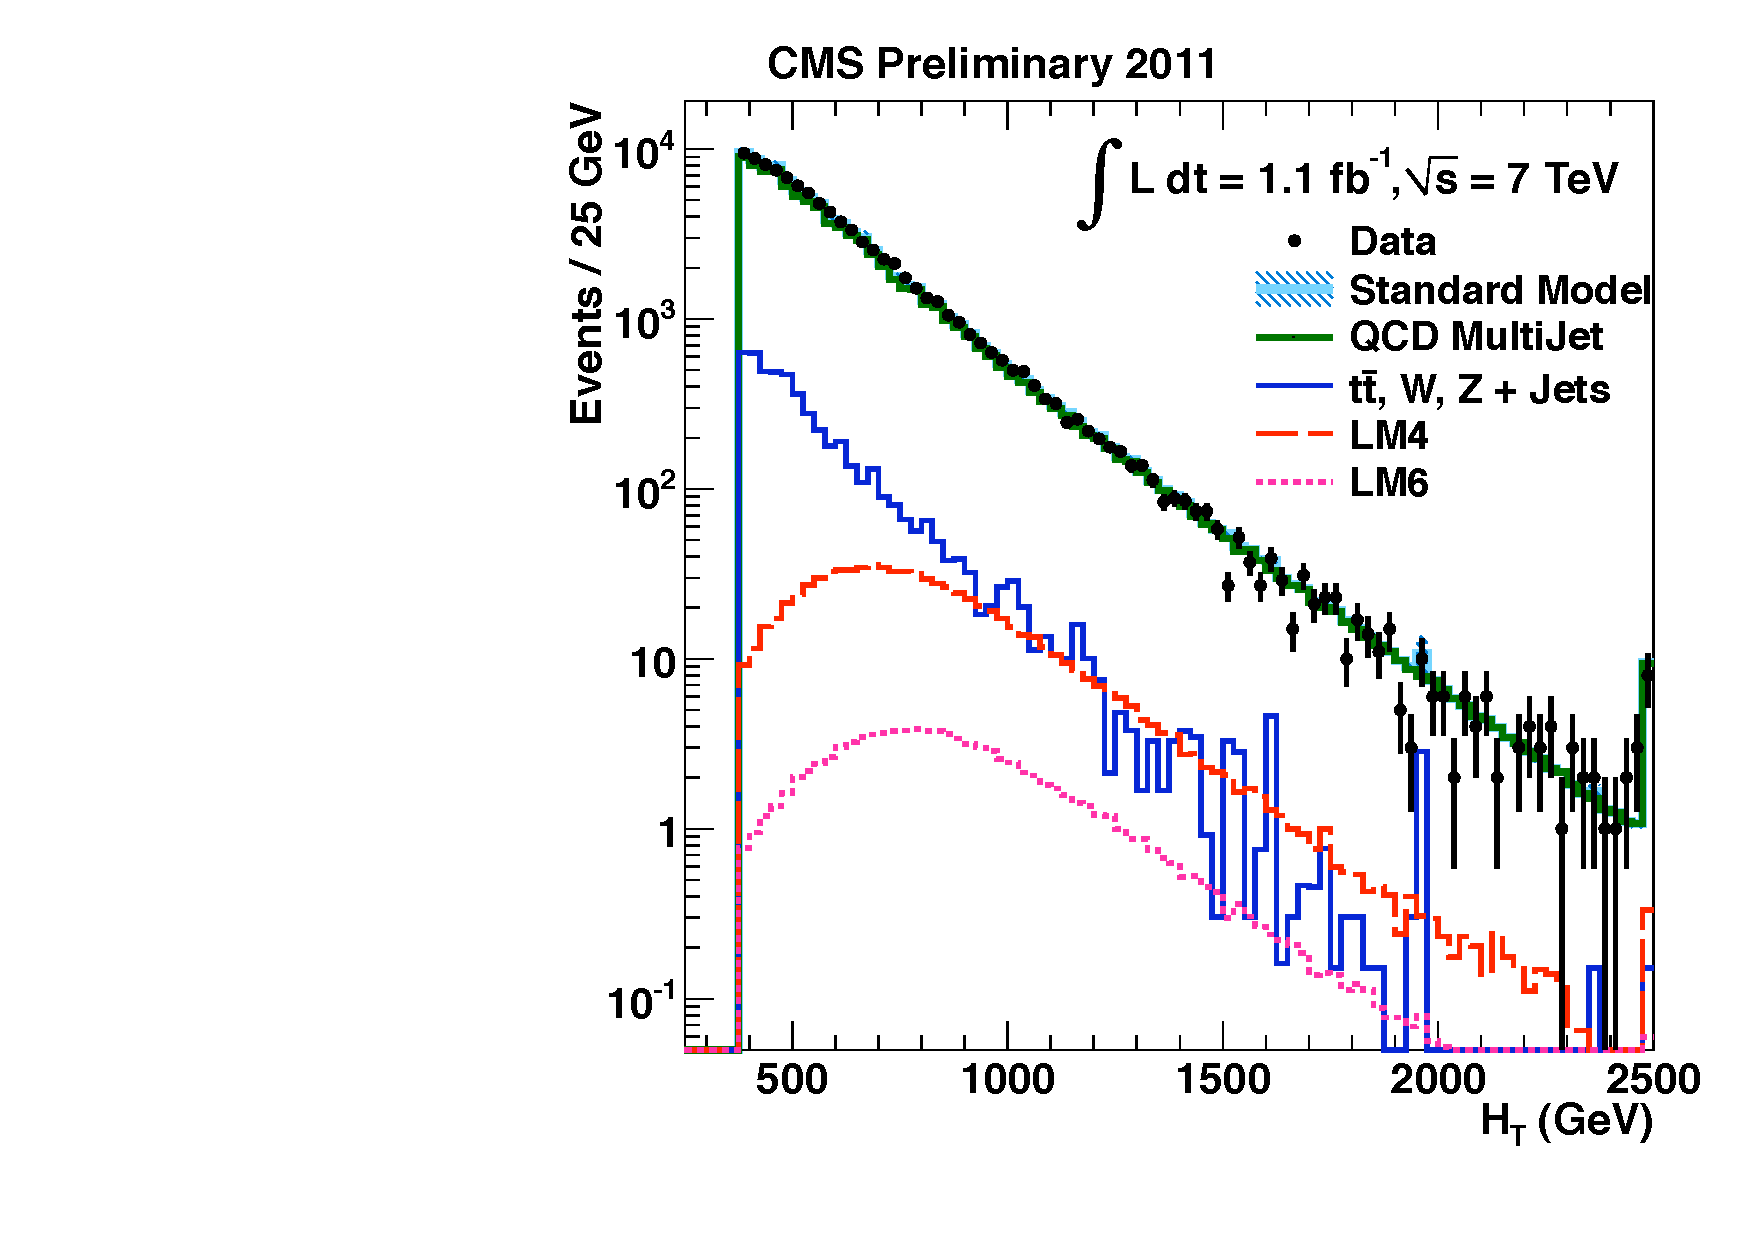
\includegraphics[width=0.40\textwidth]{Figures/Analysis/PAS/HT_all.pdf}}
\subfigure[Comparison of the jet multiplicity between data and MC for the hadronic selection, for $H_{T}$ $\geq$ 375 GeV and MHT $>$ 100 GeV.]{\label{fig:figures_JetMultiplicity_all}
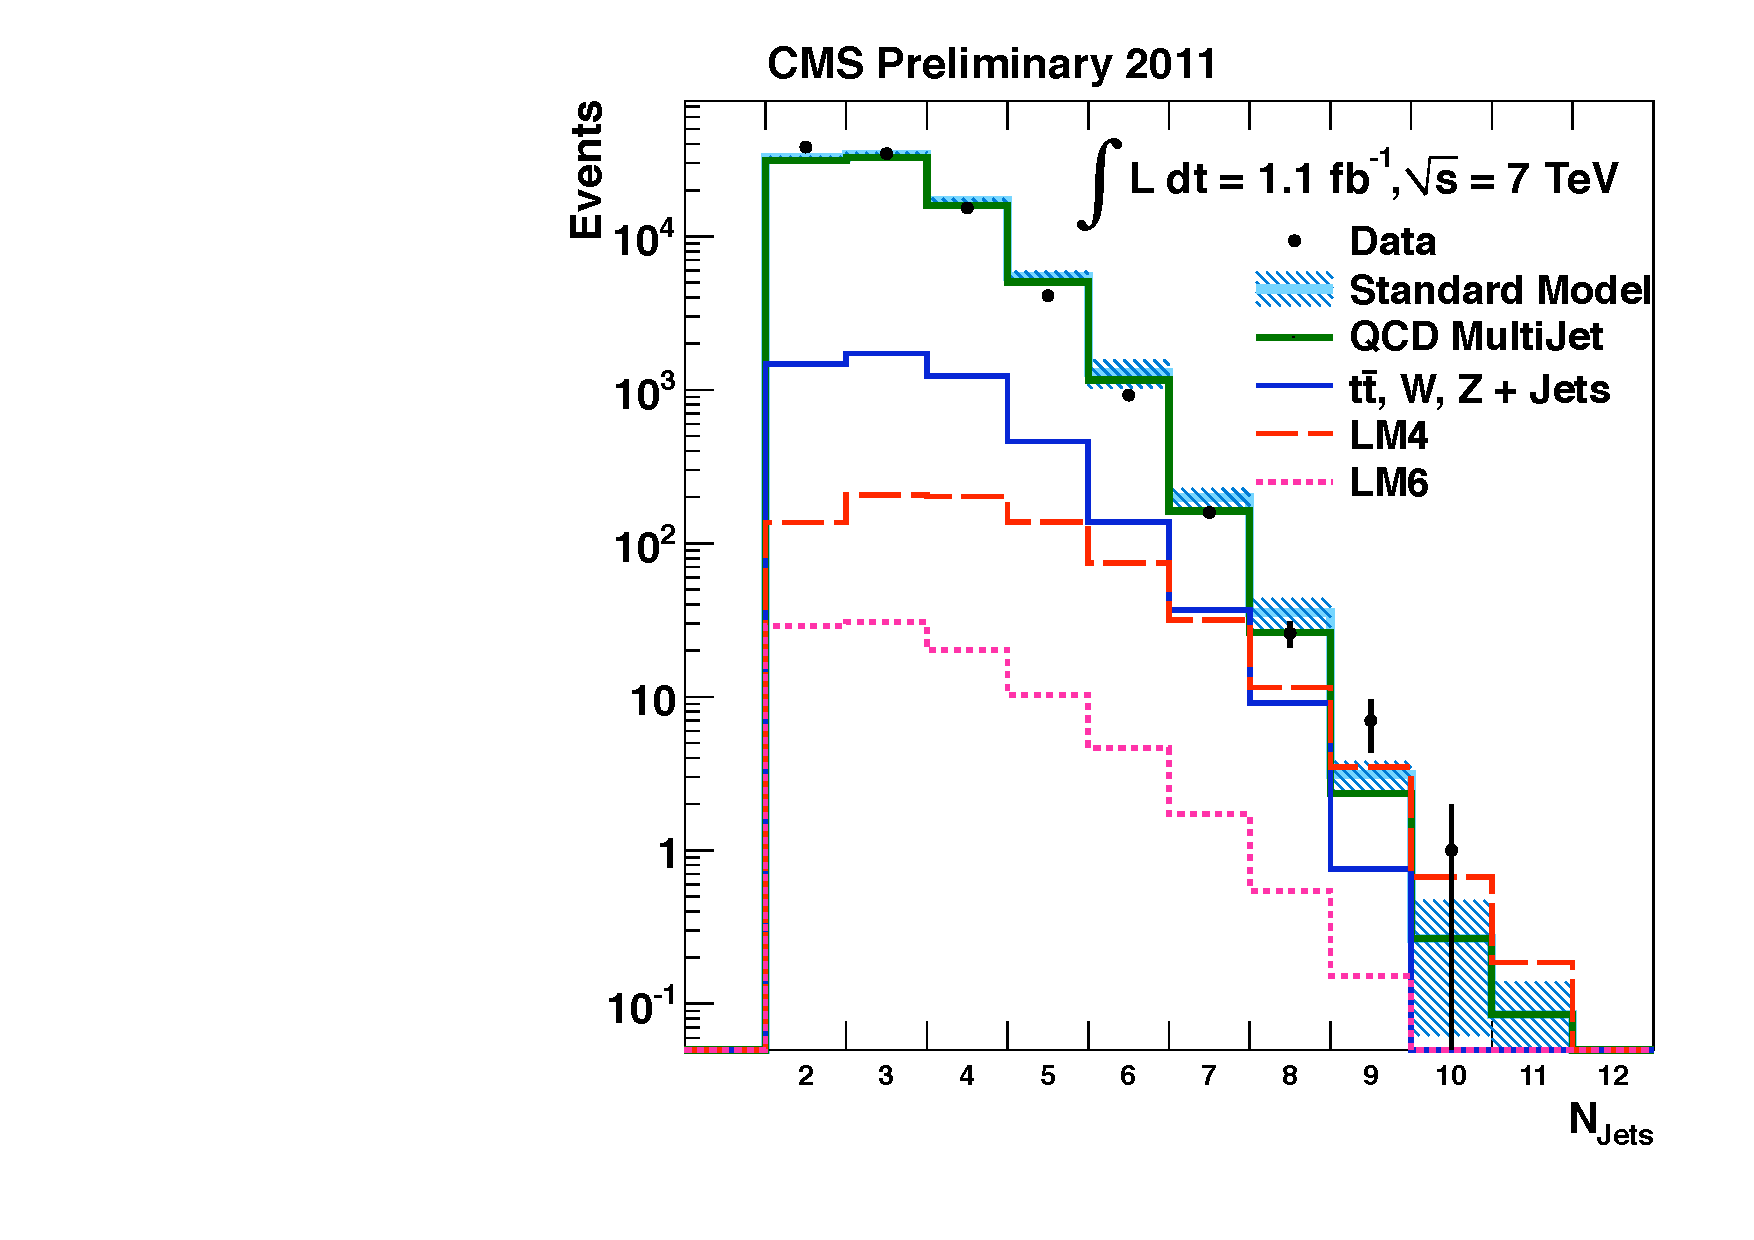
\includegraphics[width=0.40\textwidth]{Figures/Analysis/PAS/JetMultiplicity_all.pdf}
}
 \newline
\subfigure[Comparison of the $\alpha_{T}$ distribution between data and MC for the hadronic selection, for $H_{T}$ $\geq$ 375 GeV and MHT $>$ 100 GeV.
]{\label{fig:figures_AlphaT_all}
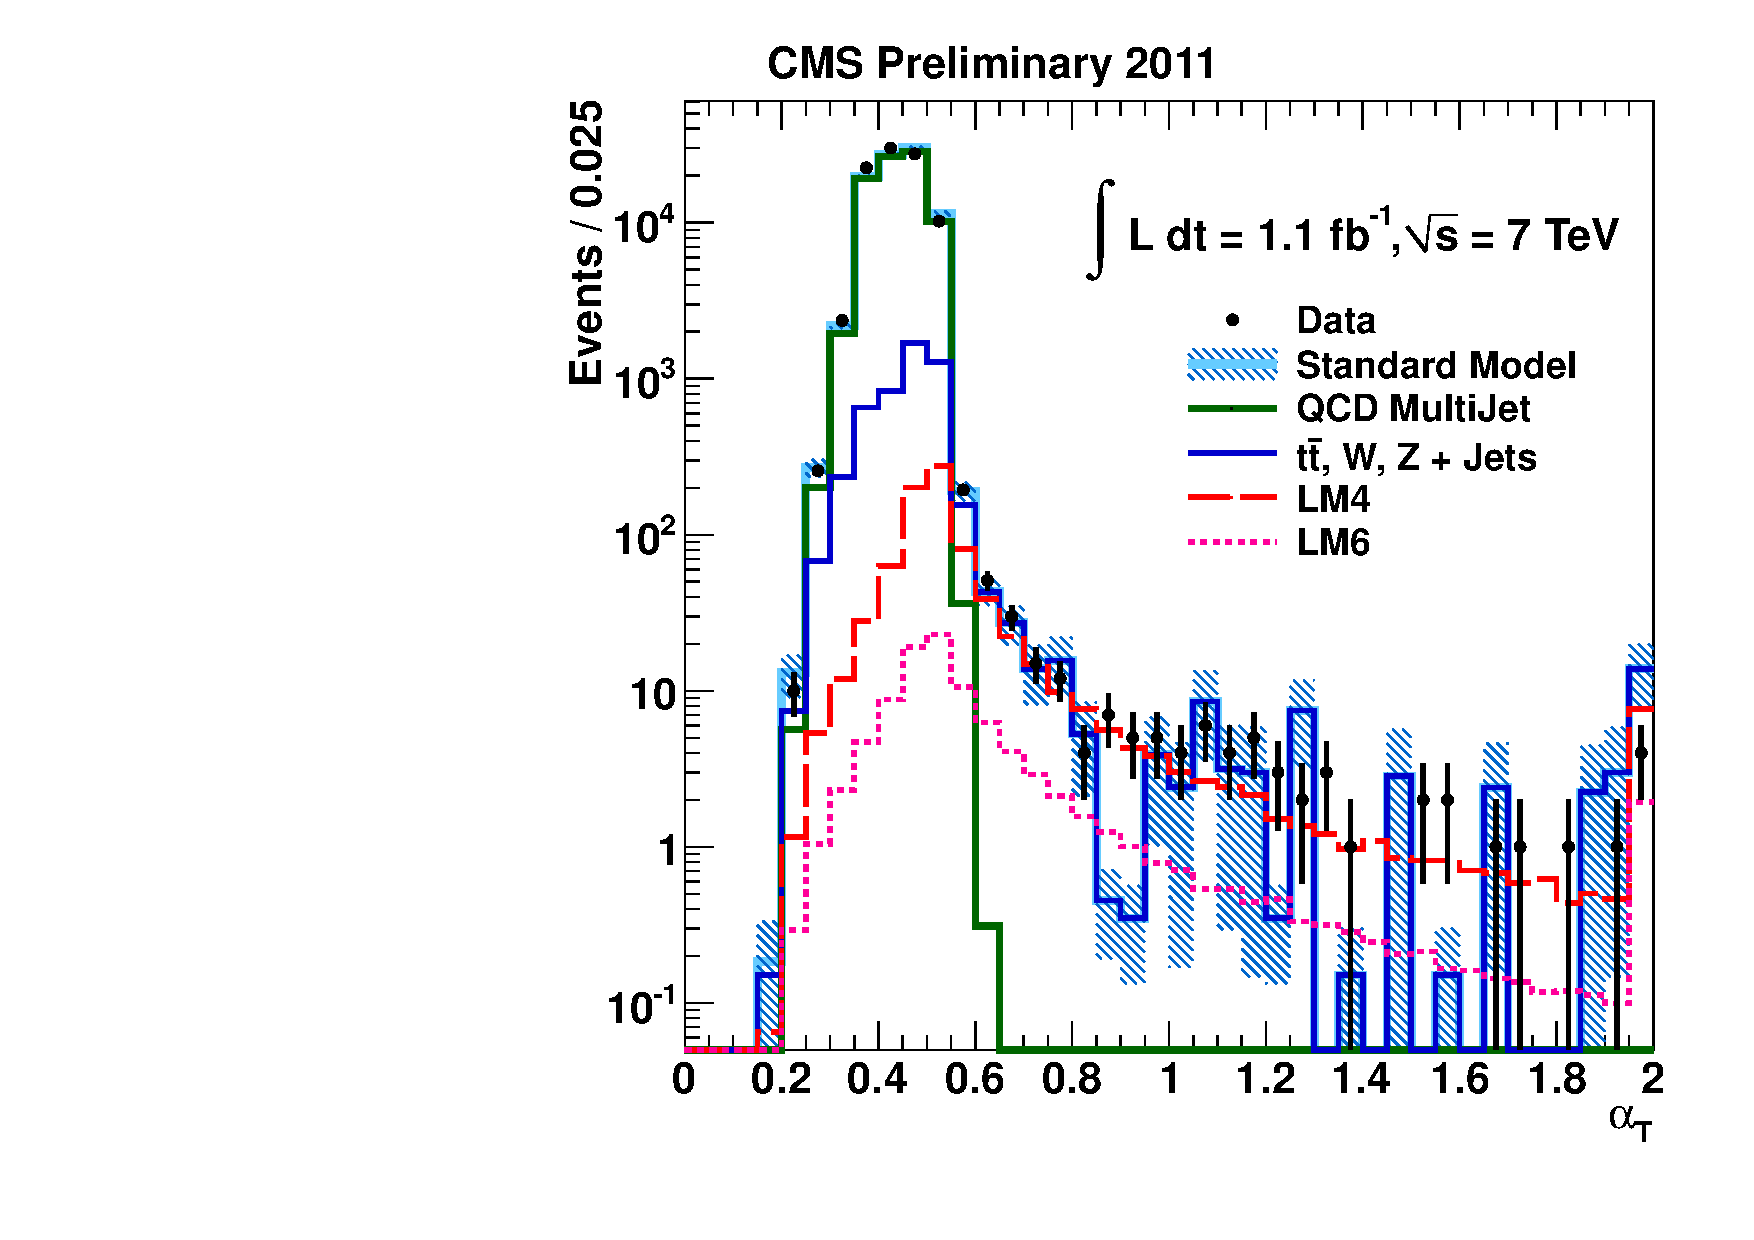
\includegraphics[width=0.40\textwidth]{Figures/Analysis/PAS/AlphaT_all.pdf}
}
\hspace{0.3cm}
  \subfigure[Comparison of the $\alpha_{T}$ distribution highlighting the agreement on the sharply falling edge between Data and Monte Carlo for the hadronic selection, in the region $H_{T}$ $\geq$ 375 GeV.]{\label{fig:figures_AlphaT_Zoomed_all}
          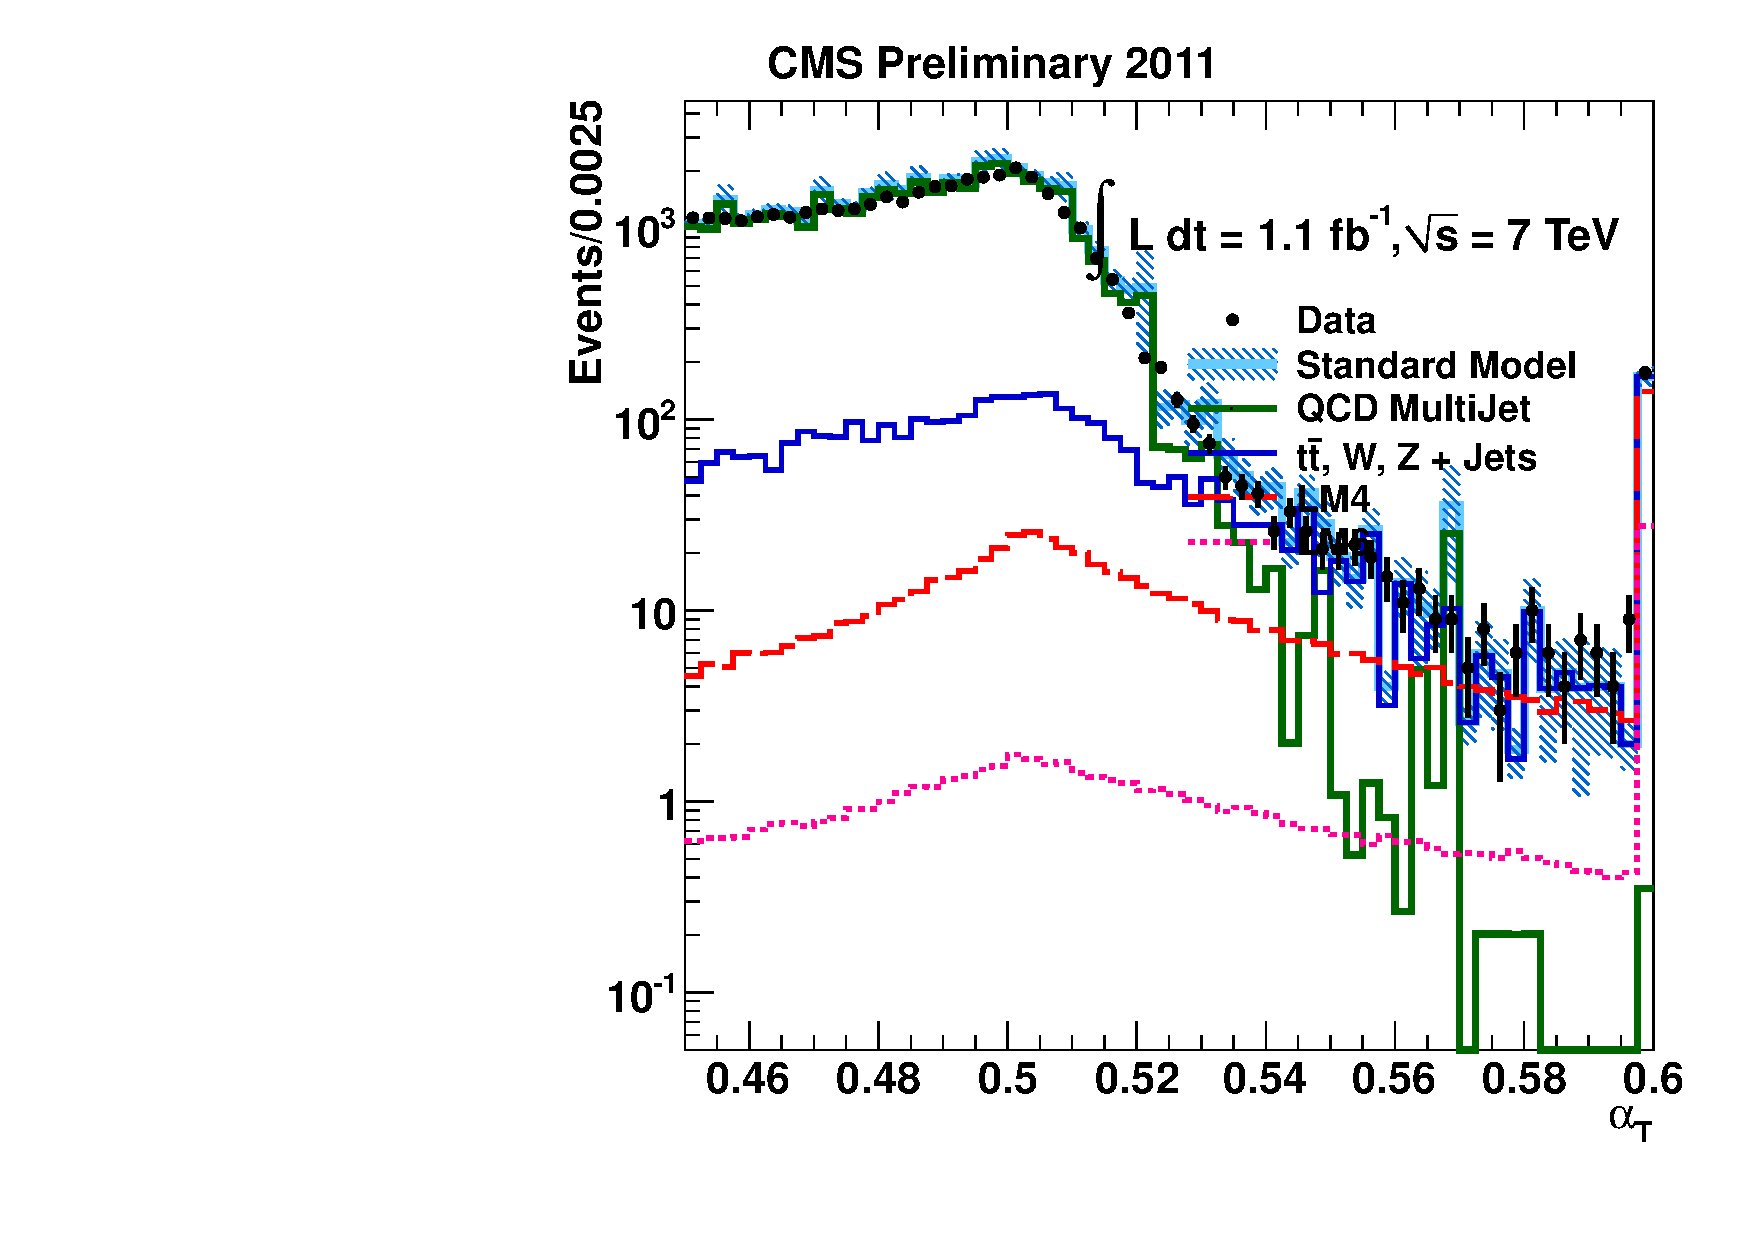
\includegraphics[width=0.40\textwidth]{Figures/Analysis/PAS/AlphaT_Zoomed_all.pdf}
     }
    \caption{Comparisons of 1.1 \fb 2011 7TeV CMS Data and equivalently weighted Monte-Carlo in basic kinematic quantities prior to the $\alpha_{T}$ selection cut.}
\end{figure}
\begin{figure}[h]
    \centering
     \subfigure[$\Delta \Phi^{*}$ distribution after $\alpha_{T}$ selection.]{
          \label{fig:BiasedDeltaPhi_after_alphaT_55_all}
          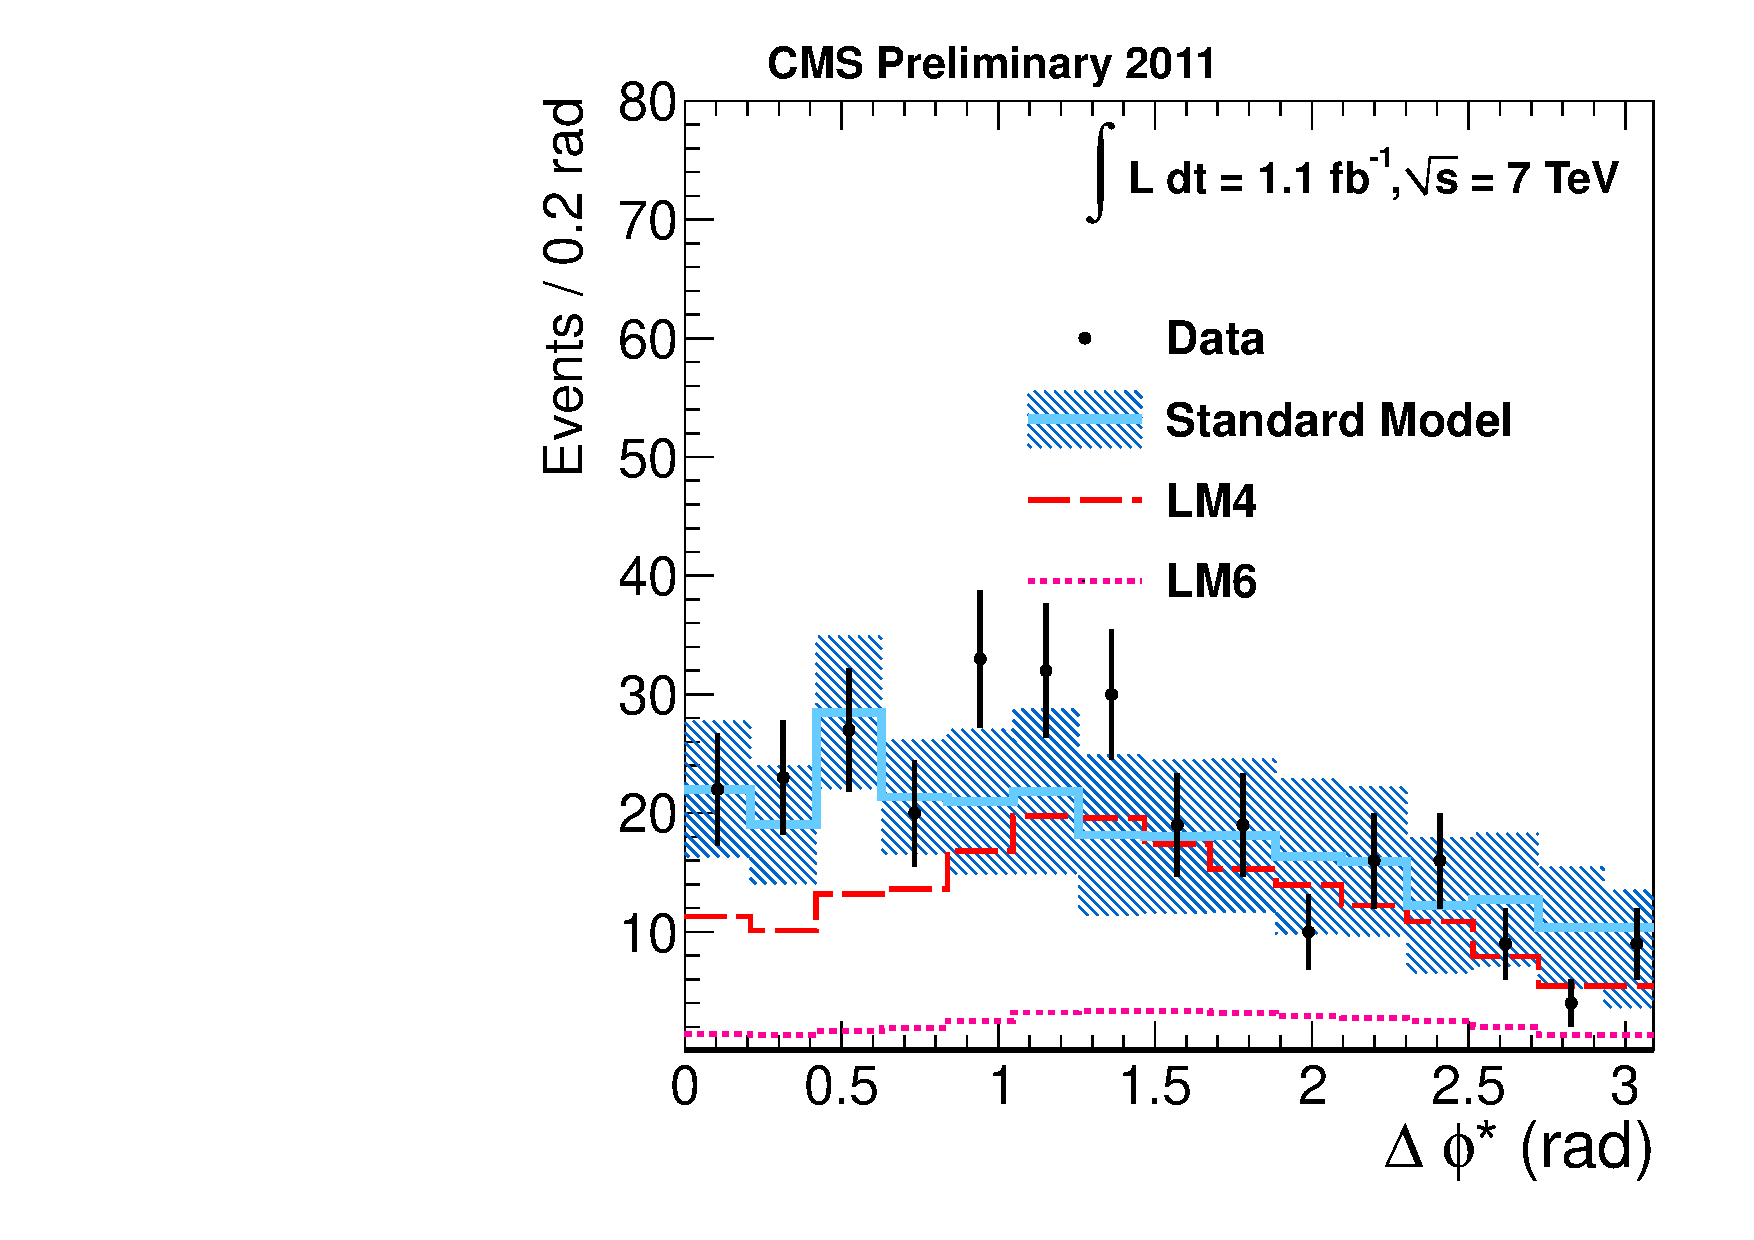
\includegraphics[width=0.46\textwidth]{Figures/Analysis/PAS/BiasedDeltaPhi_after_alphaT_55_all.pdf}
     }
\hspace{0.3cm}
    \subfigure[The effective mass distribution, $M_{\rm eff}$ = $H_{T}$ +
    MHT, of the events passing the $\alpha_{T}$ selection.]{
          \label{fig:EffectiveMass_after_alphaT_55_all}
          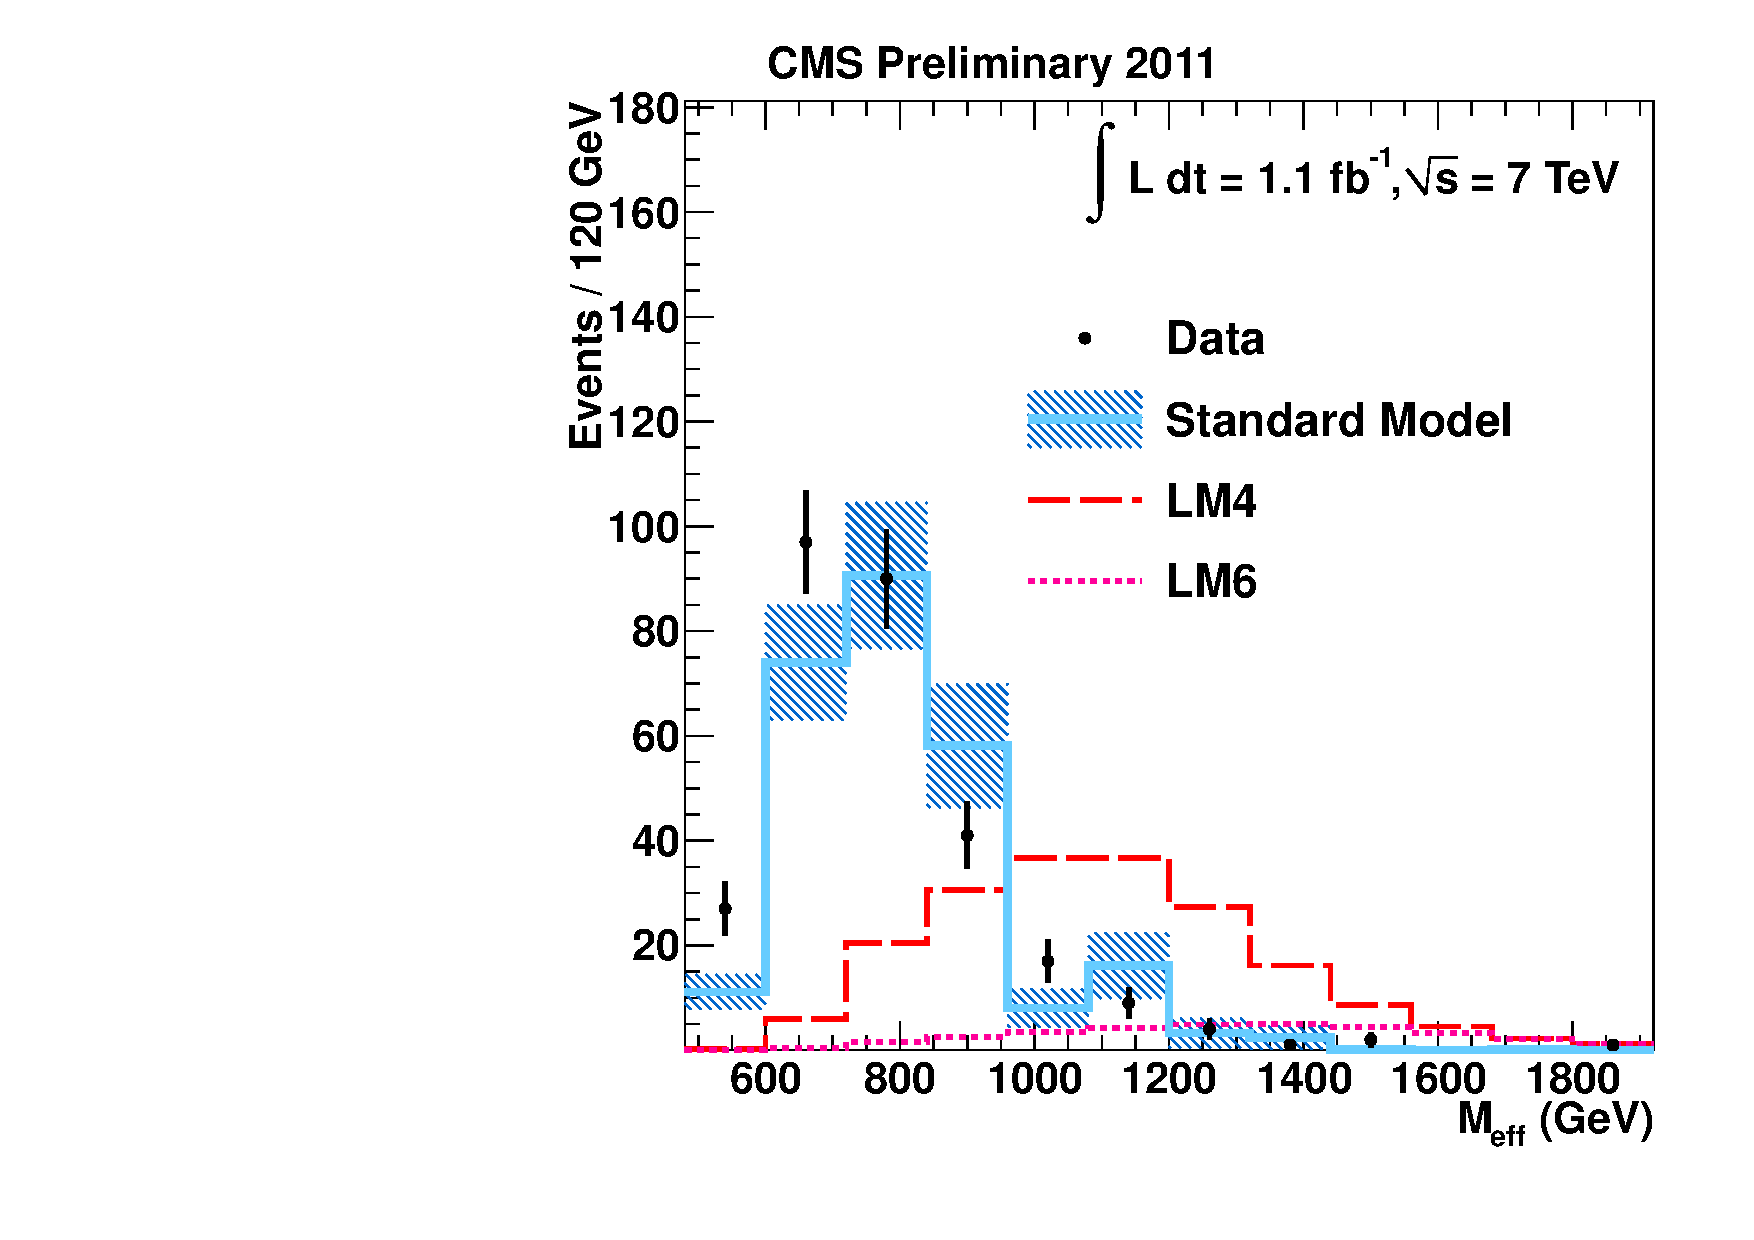
\includegraphics[width=0.46\textwidth]{Figures/Analysis/PAS/EffectiveMass_after_alphaT_55_all.pdf}
     }
    \newline
    \subfigure[Jet multiplicity after $\alpha_{T}$ selection.]{
          \label{fig:JetMultiplicityAfterAlphaT_all}
          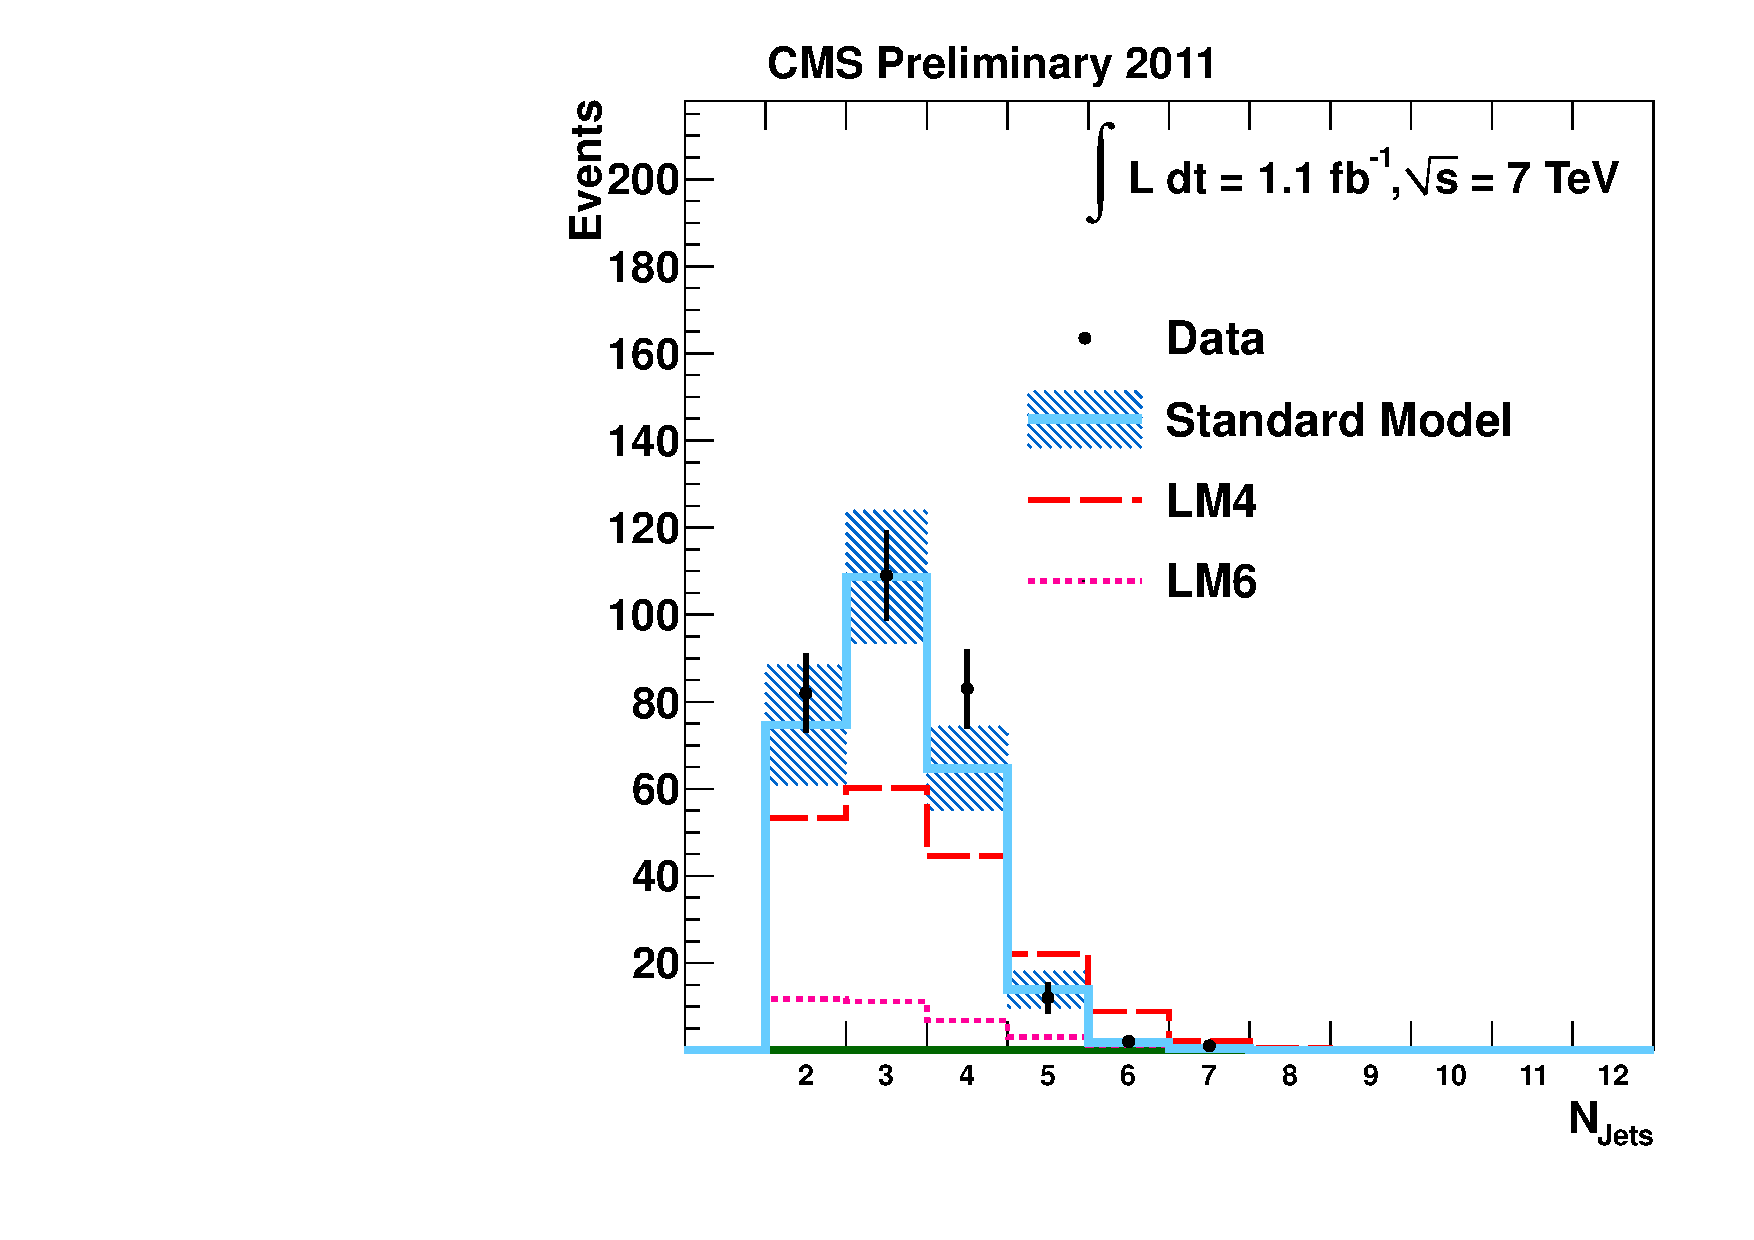
\includegraphics[width=0.46\textwidth]{Figures/Analysis/PAS/JetMultiplicityAfterAlphaT_all.pdf}
     }
\caption{Comparisons of 1.1 \fb 2011 7TeV CMS Data and equivalently weighted Monte-Carlo in basic kinematic quantities after the $\alpha_{T}$ selection cut.}
\end{figure}

\subsection{Dependence of $R_{\alpha_{T}}$ on $H_{T}$}




\begin{figure}[h]
  \begin{center}
    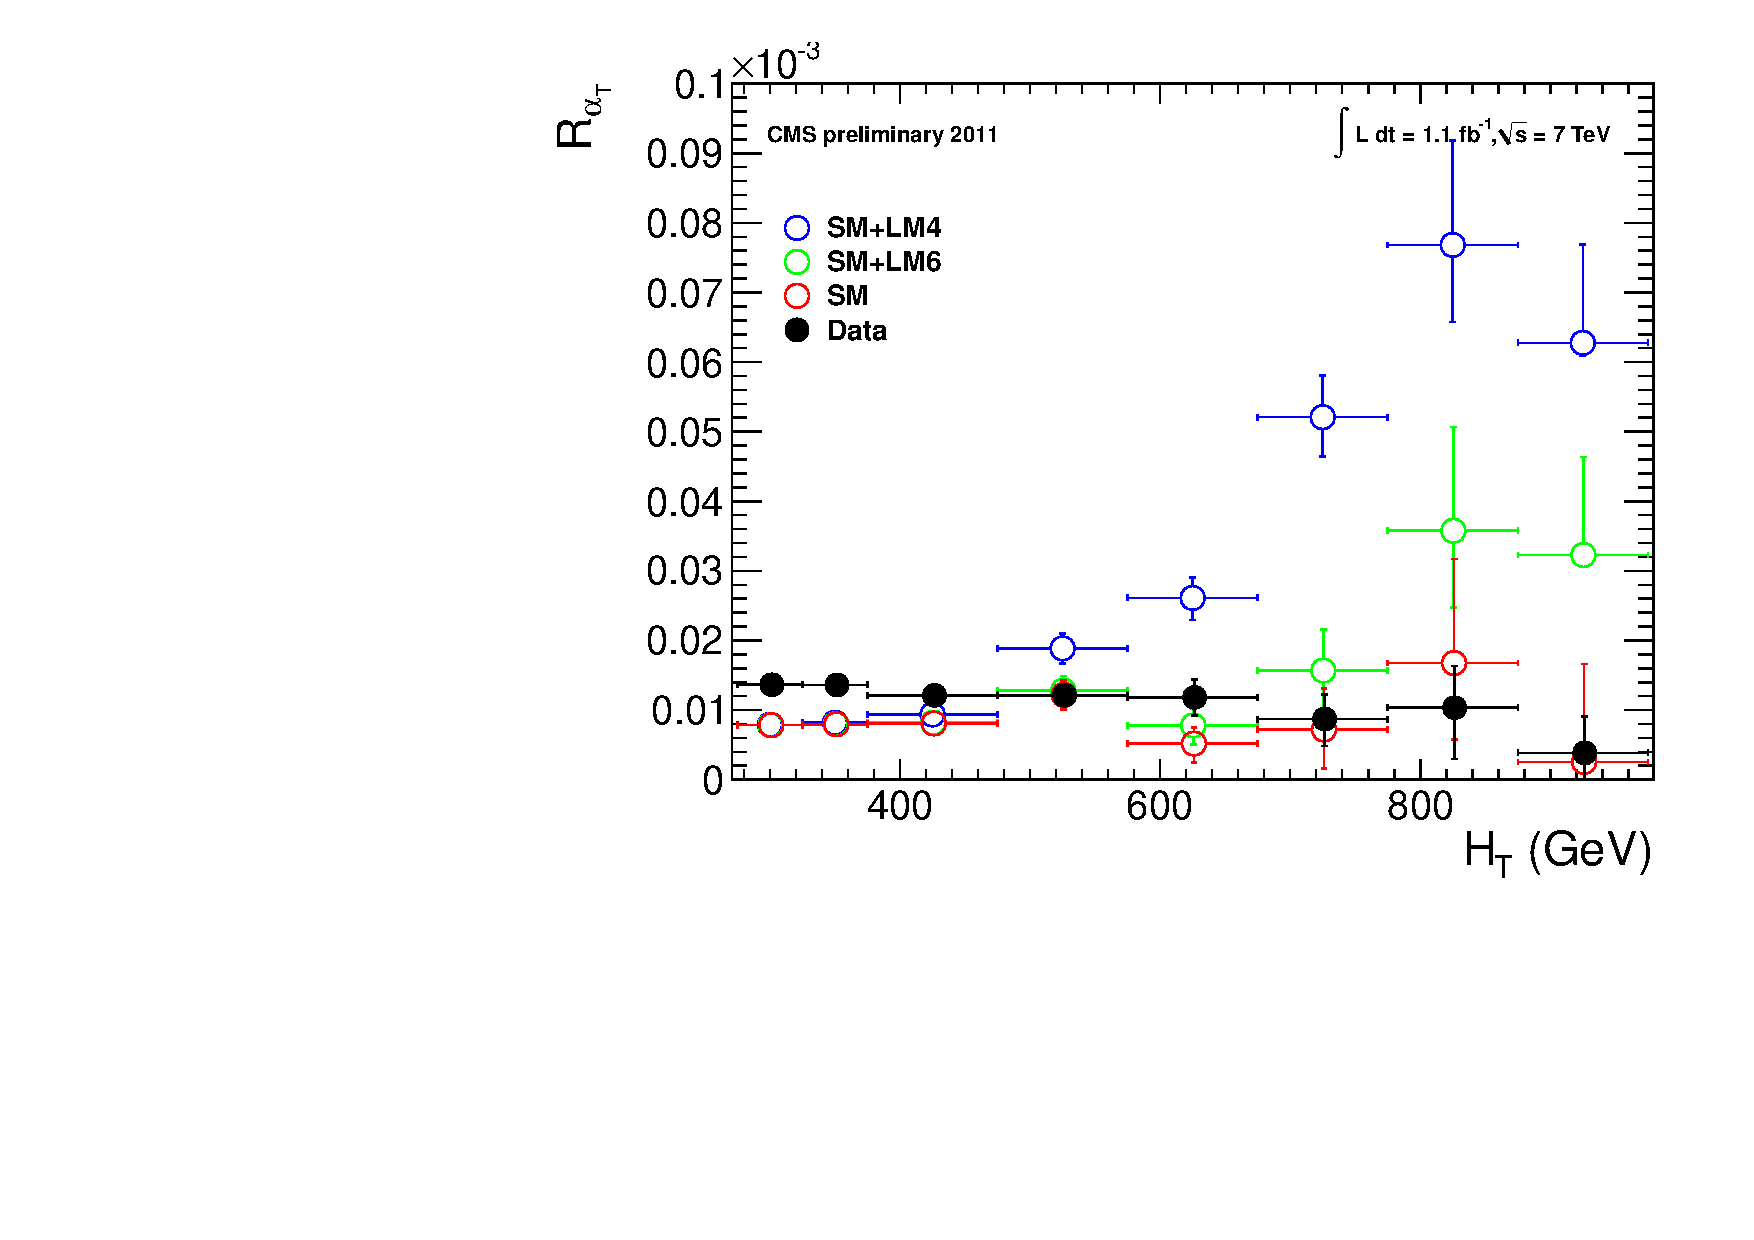
\includegraphics[width = 0.48\textwidth]{Figures/Analysis/PAS/Ratio_Multi2Incl_AlphaT55.pdf}
    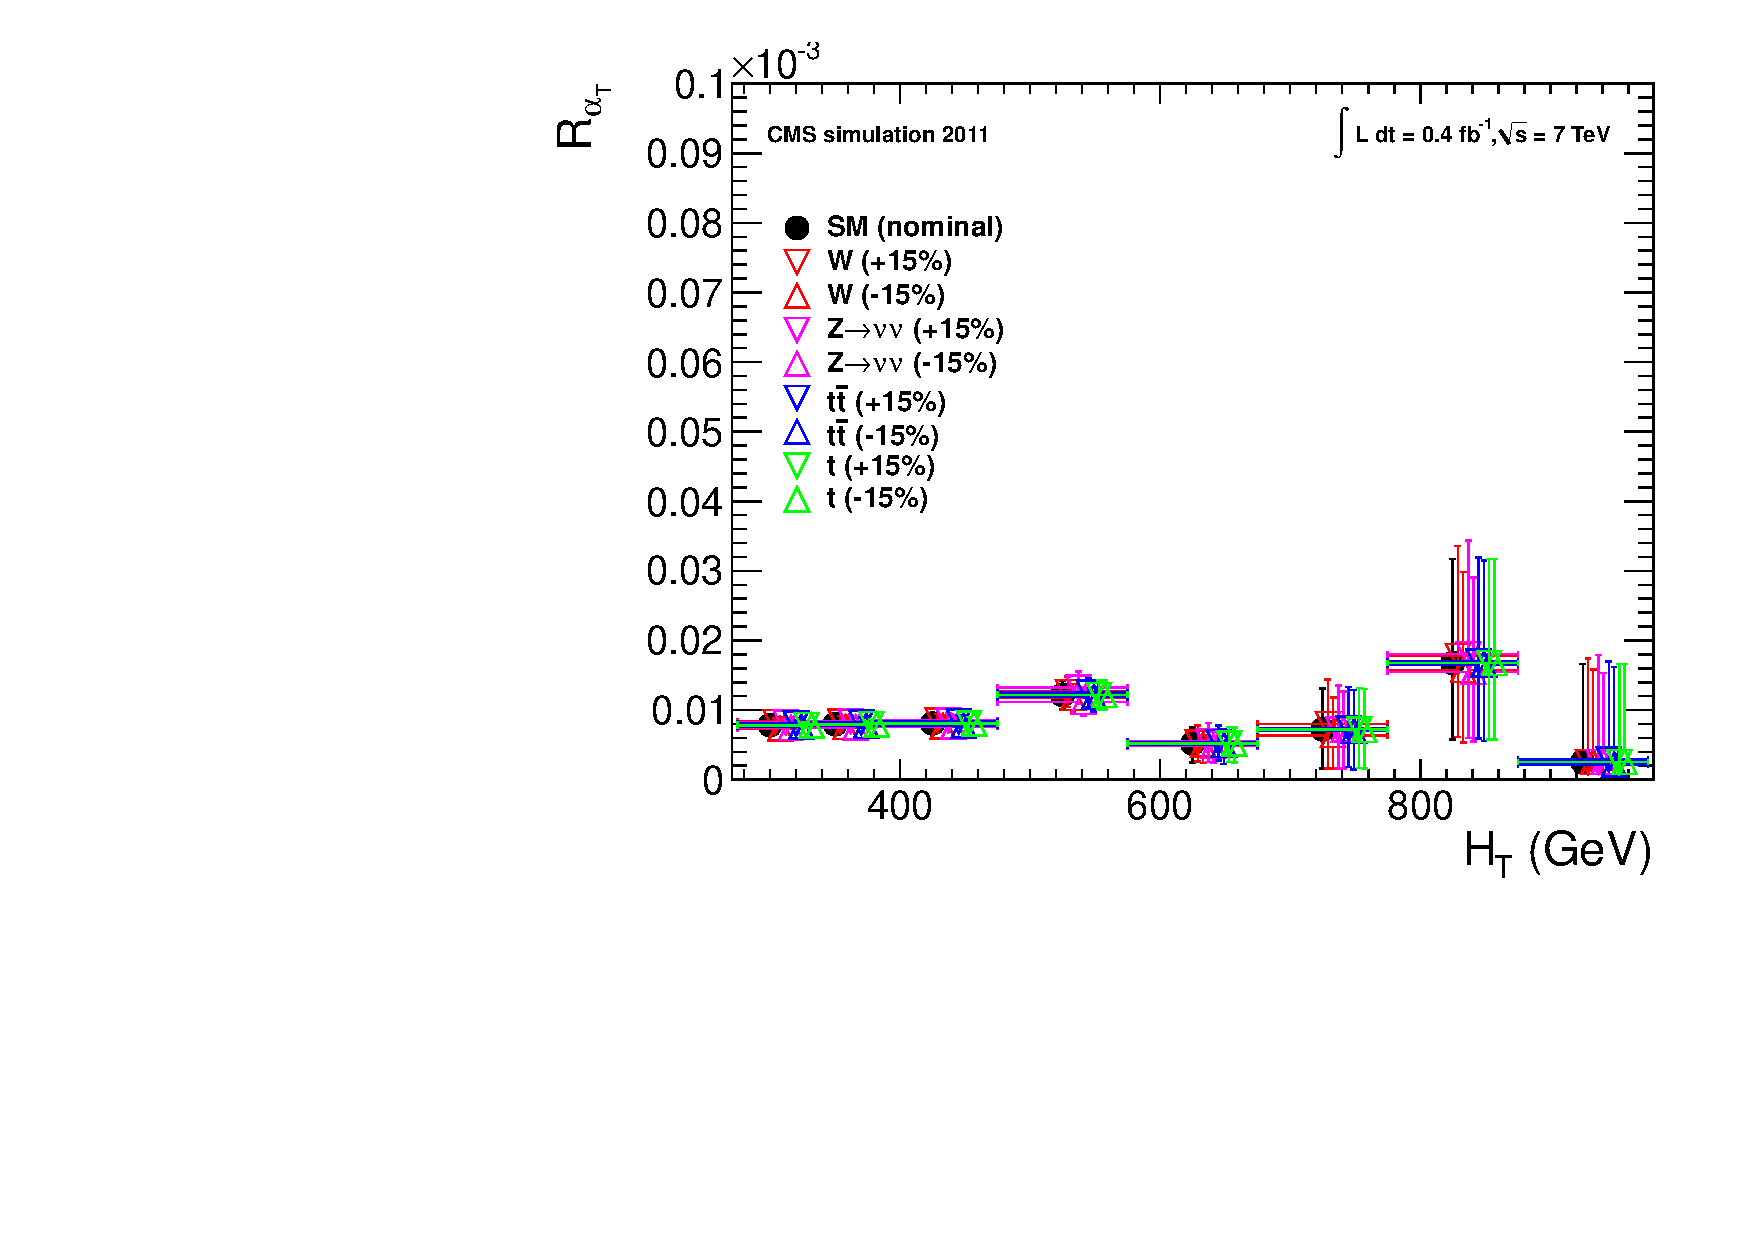
\includegraphics[width = 0.48\textwidth]{Figures/Analysis/PAS/Syst_Multi2Incl_AlphaT55.pdf}
    \caption{\label{fig:rat_vs_ht} (Left) The dependence of \RaT on
      \HT for events with N$_{\mathrm{jet}} \geq 2$. (Right) Dependence of rat on
      \HT when varying the effective cross-section of the four major
      EWK background components individually by $\pm$15\%. (Markers
      are artificially offset for clarity.)  }
  \end{center}
\end{figure}






\section{Data-Driven Background Estimation}
\subsection{Total background prediction}
\subsection{Estimating EWK background using high $p_{T}$ using W+Jets events}
\begin{figure}[h]
\begin{center}
\subfigure[\label{fig:muon_beforeat_mupt}]{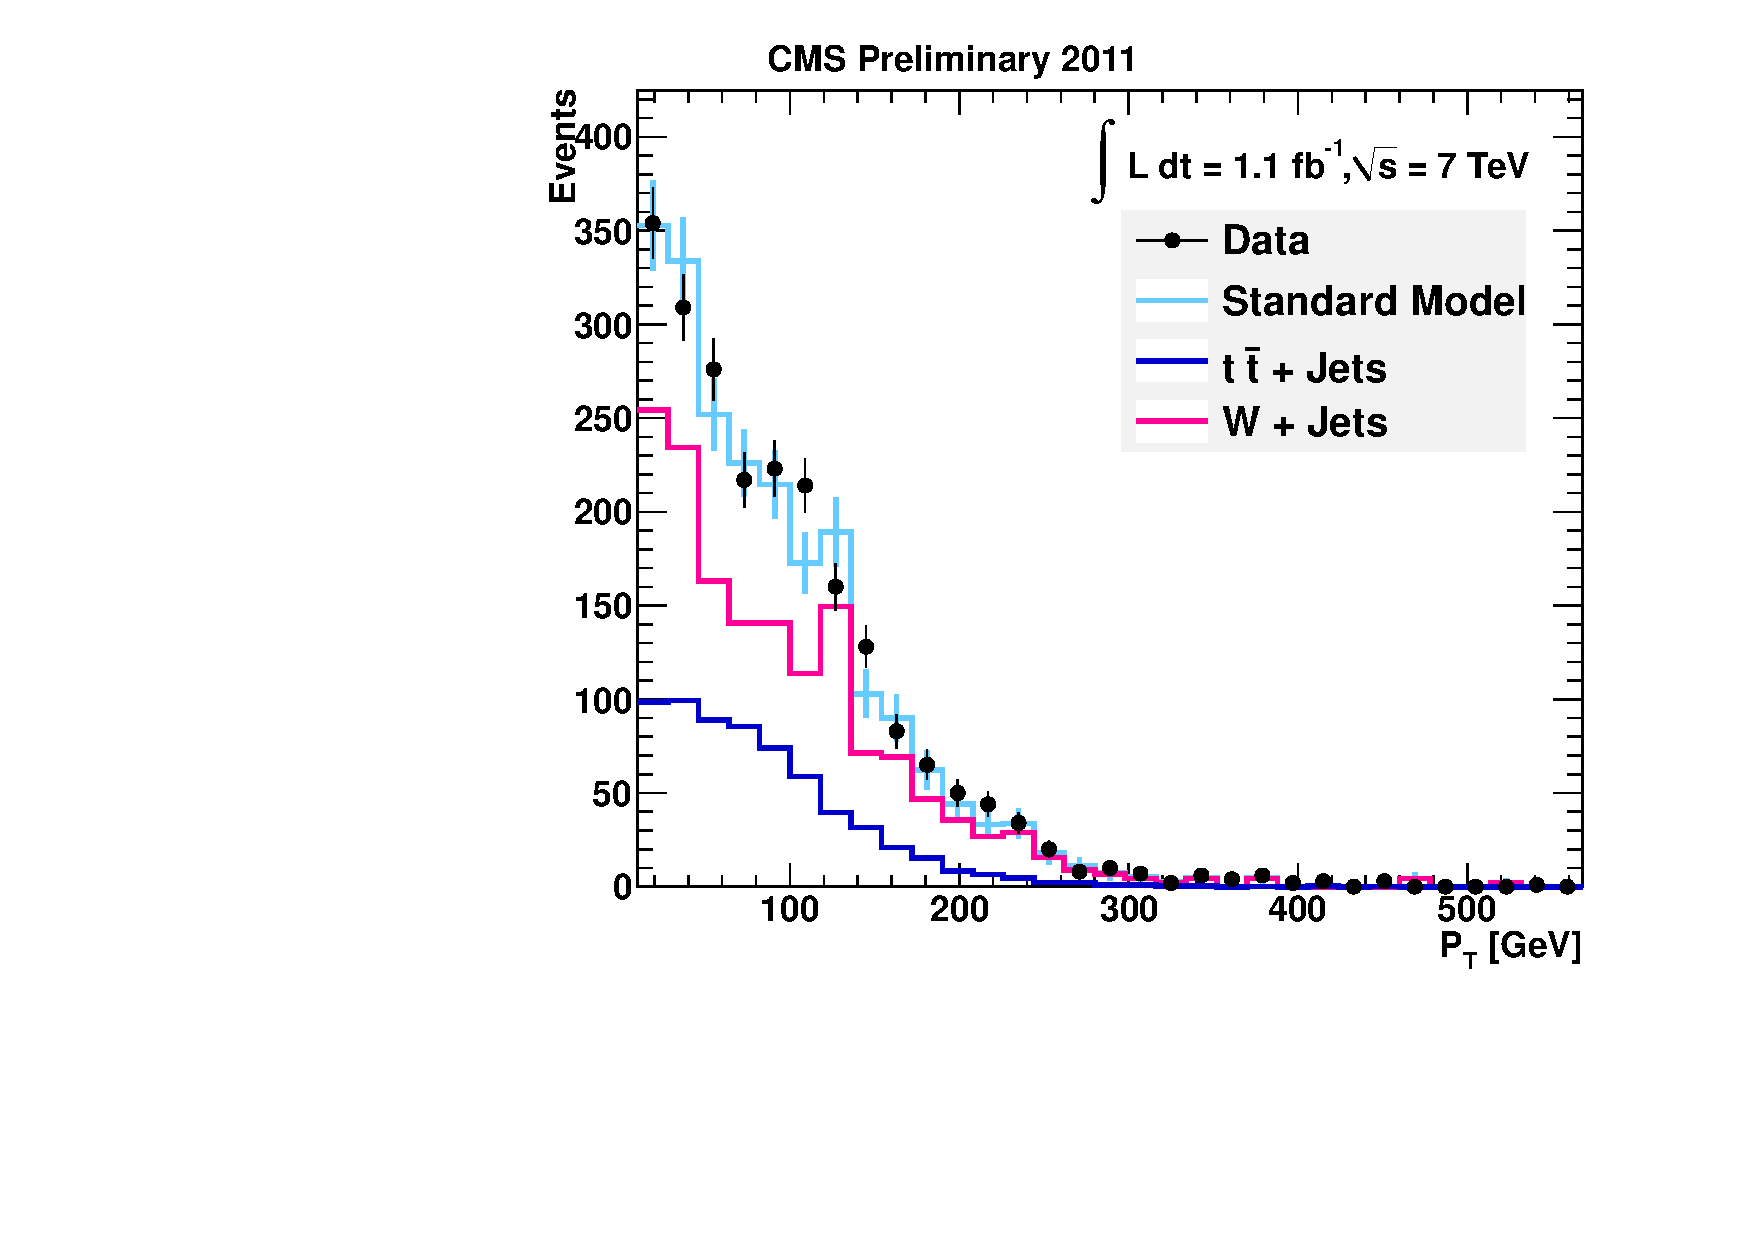
\includegraphics[width=0.45\textwidth, angle=0]{Figures/Analysis/PAS/muon_plots/spring11NoLogYMuPtMuonControl_beforeaT.pdf}}
\subfigure[\label{fig:muon_beforeat_njet}]{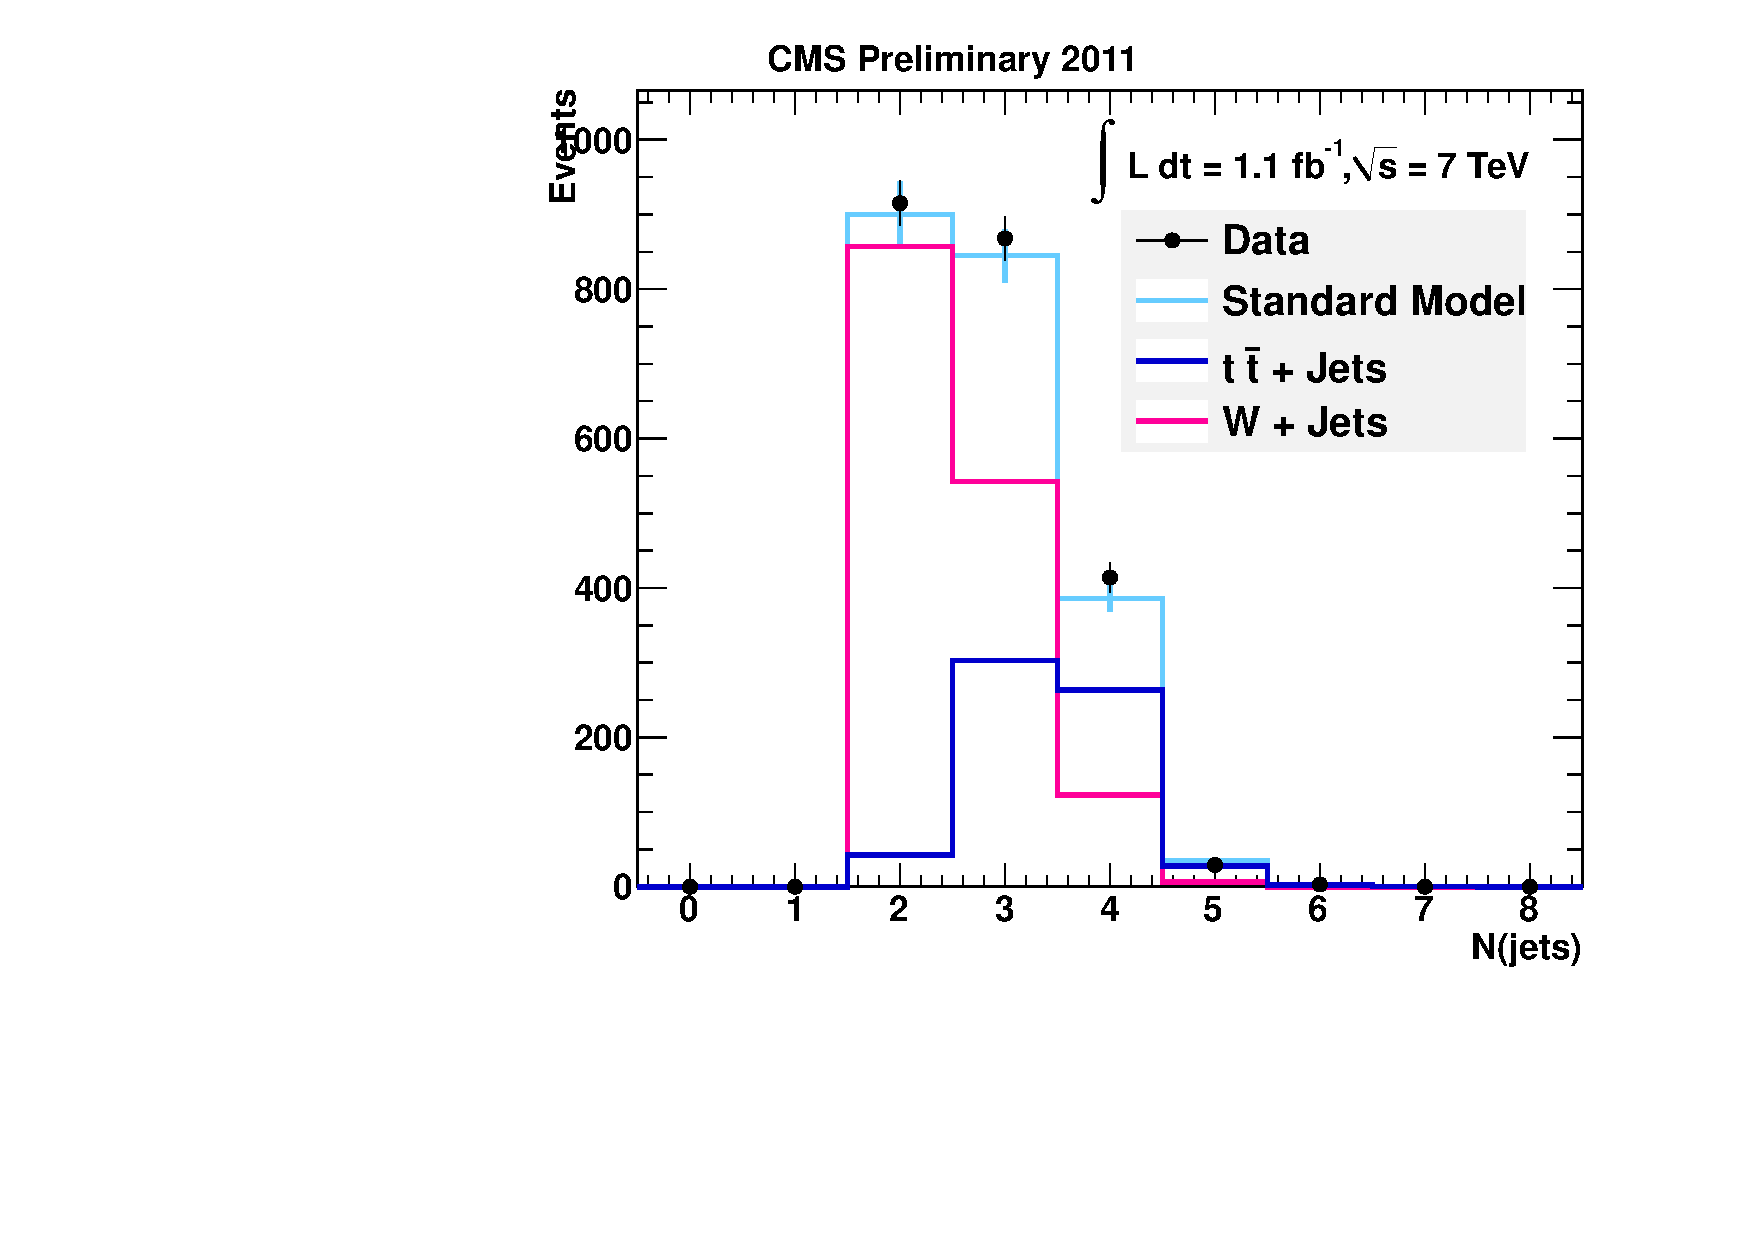
\includegraphics[width=0.45\textwidth, angle=0]{Figures/Analysis/PAS/muon_plots/spring11NoLogYnJetMuonControl_beforeaT.pdf}}
\newline
\subfigure[\label{fig:muon_beforeat_at}]{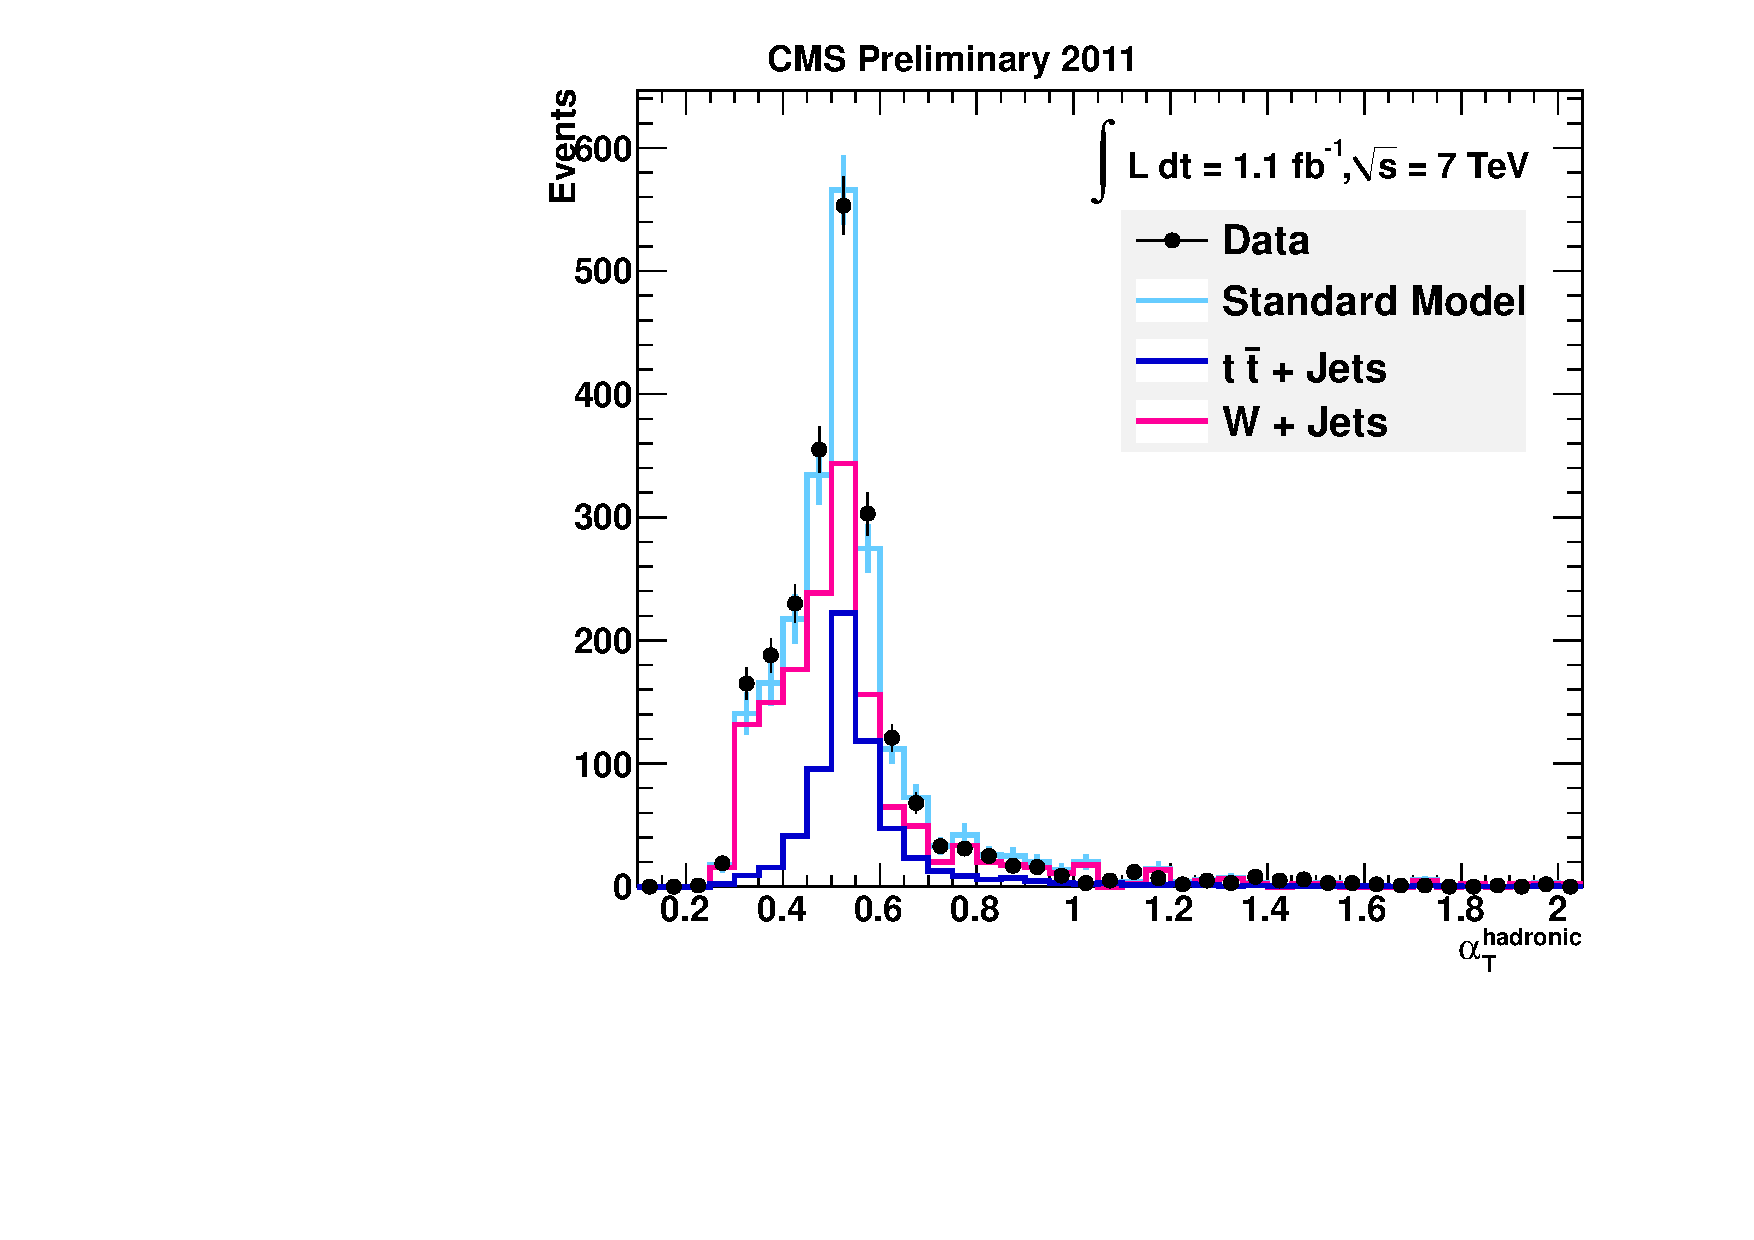
\includegraphics[width=0.45\textwidth, angle=0]{Figures/Analysis/PAS/muon_plots/spring11NoLogYaT_HMuonControl_beforeaT.pdf}}
\subfigure[\label{fig:muon_beforeat_ht}]{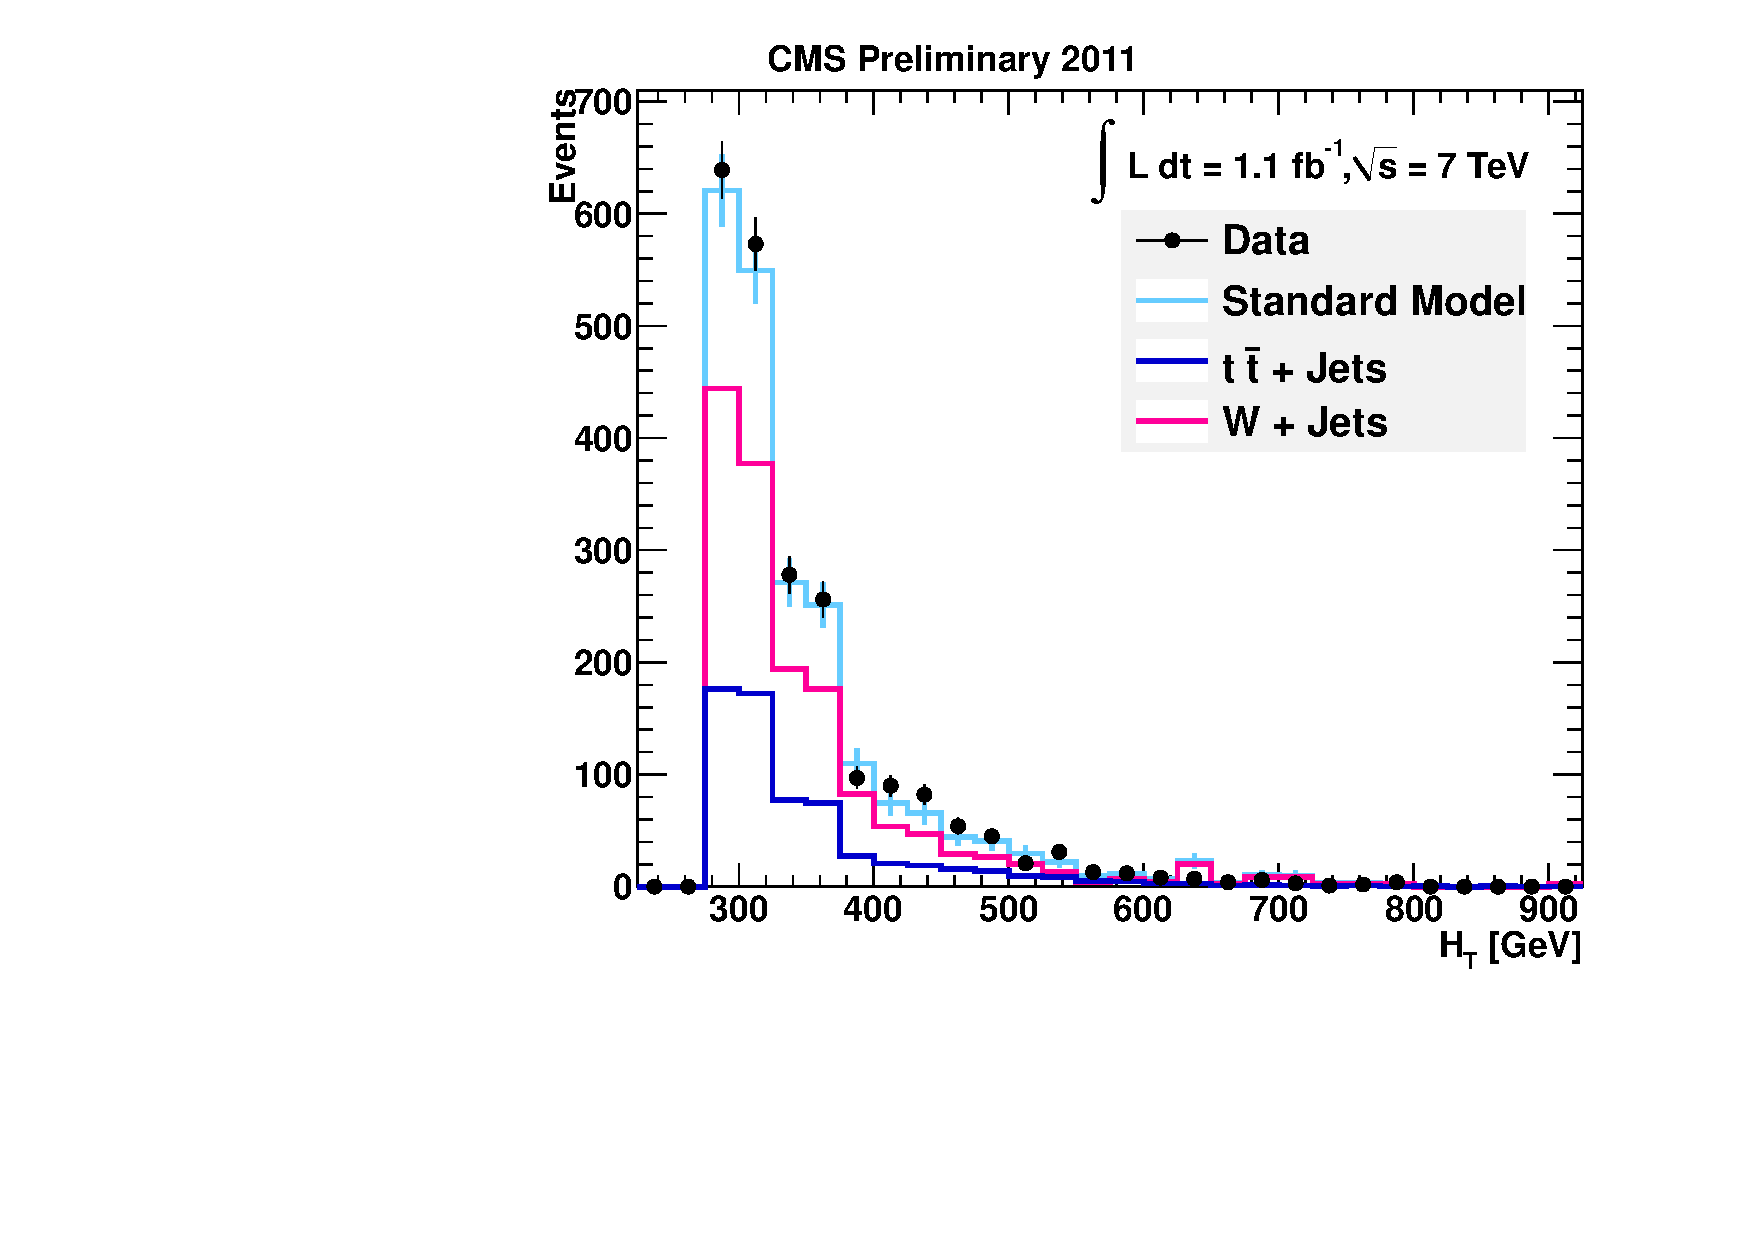
\includegraphics[width=0.45\textwidth, angle=0]{Figures/Analysis/PAS/muon_plots/spring11NoLogYHTMuonControl_beforeaT.pdf}}
\newline
\subfigure[\label{fig:muon_beforeat_MuIso}]{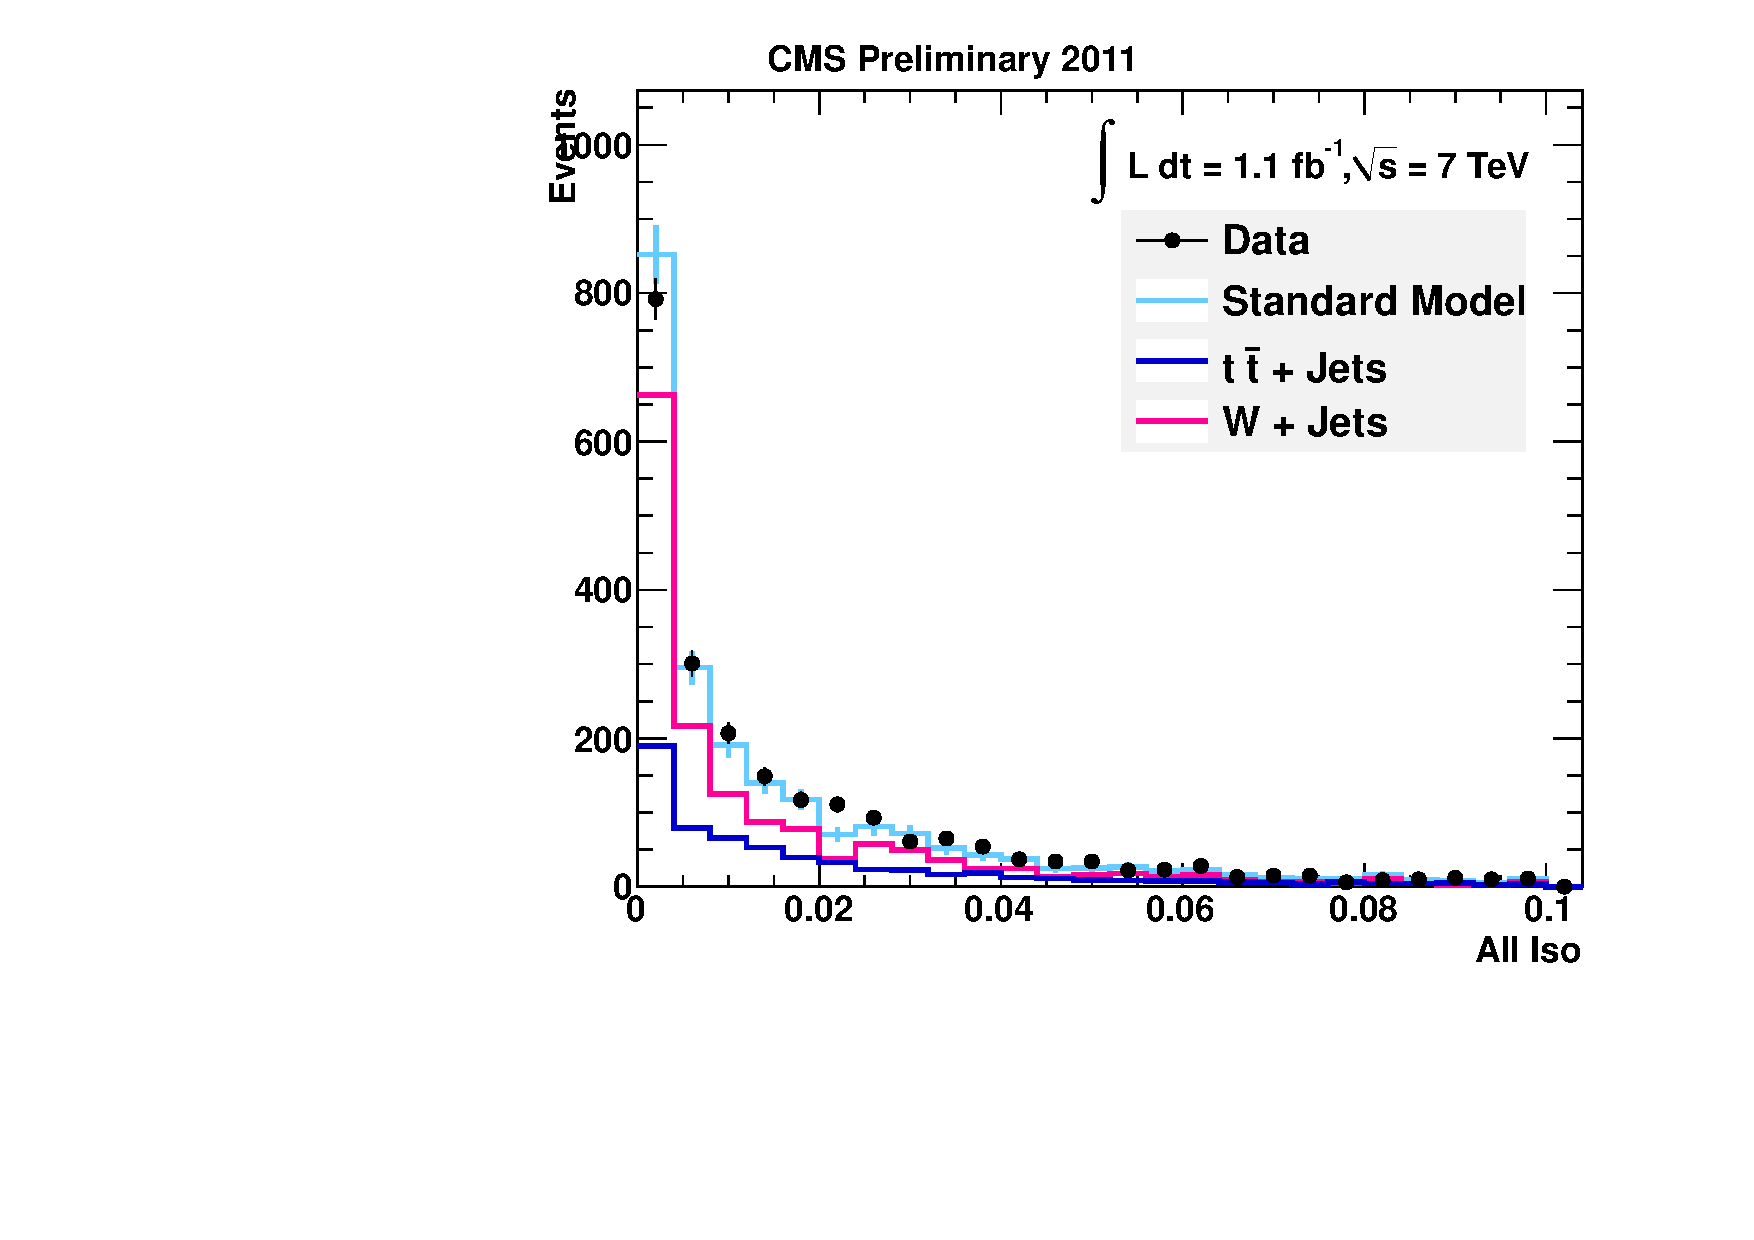
\includegraphics[width=0.45\textwidth, angle=0]{Figures/Analysis/PAS/muon_plots/spring11NoLogYMuCsoMuonControl_beforeaT.pdf}}
\subfigure[\label{fig:muon_beforeat_mt}]{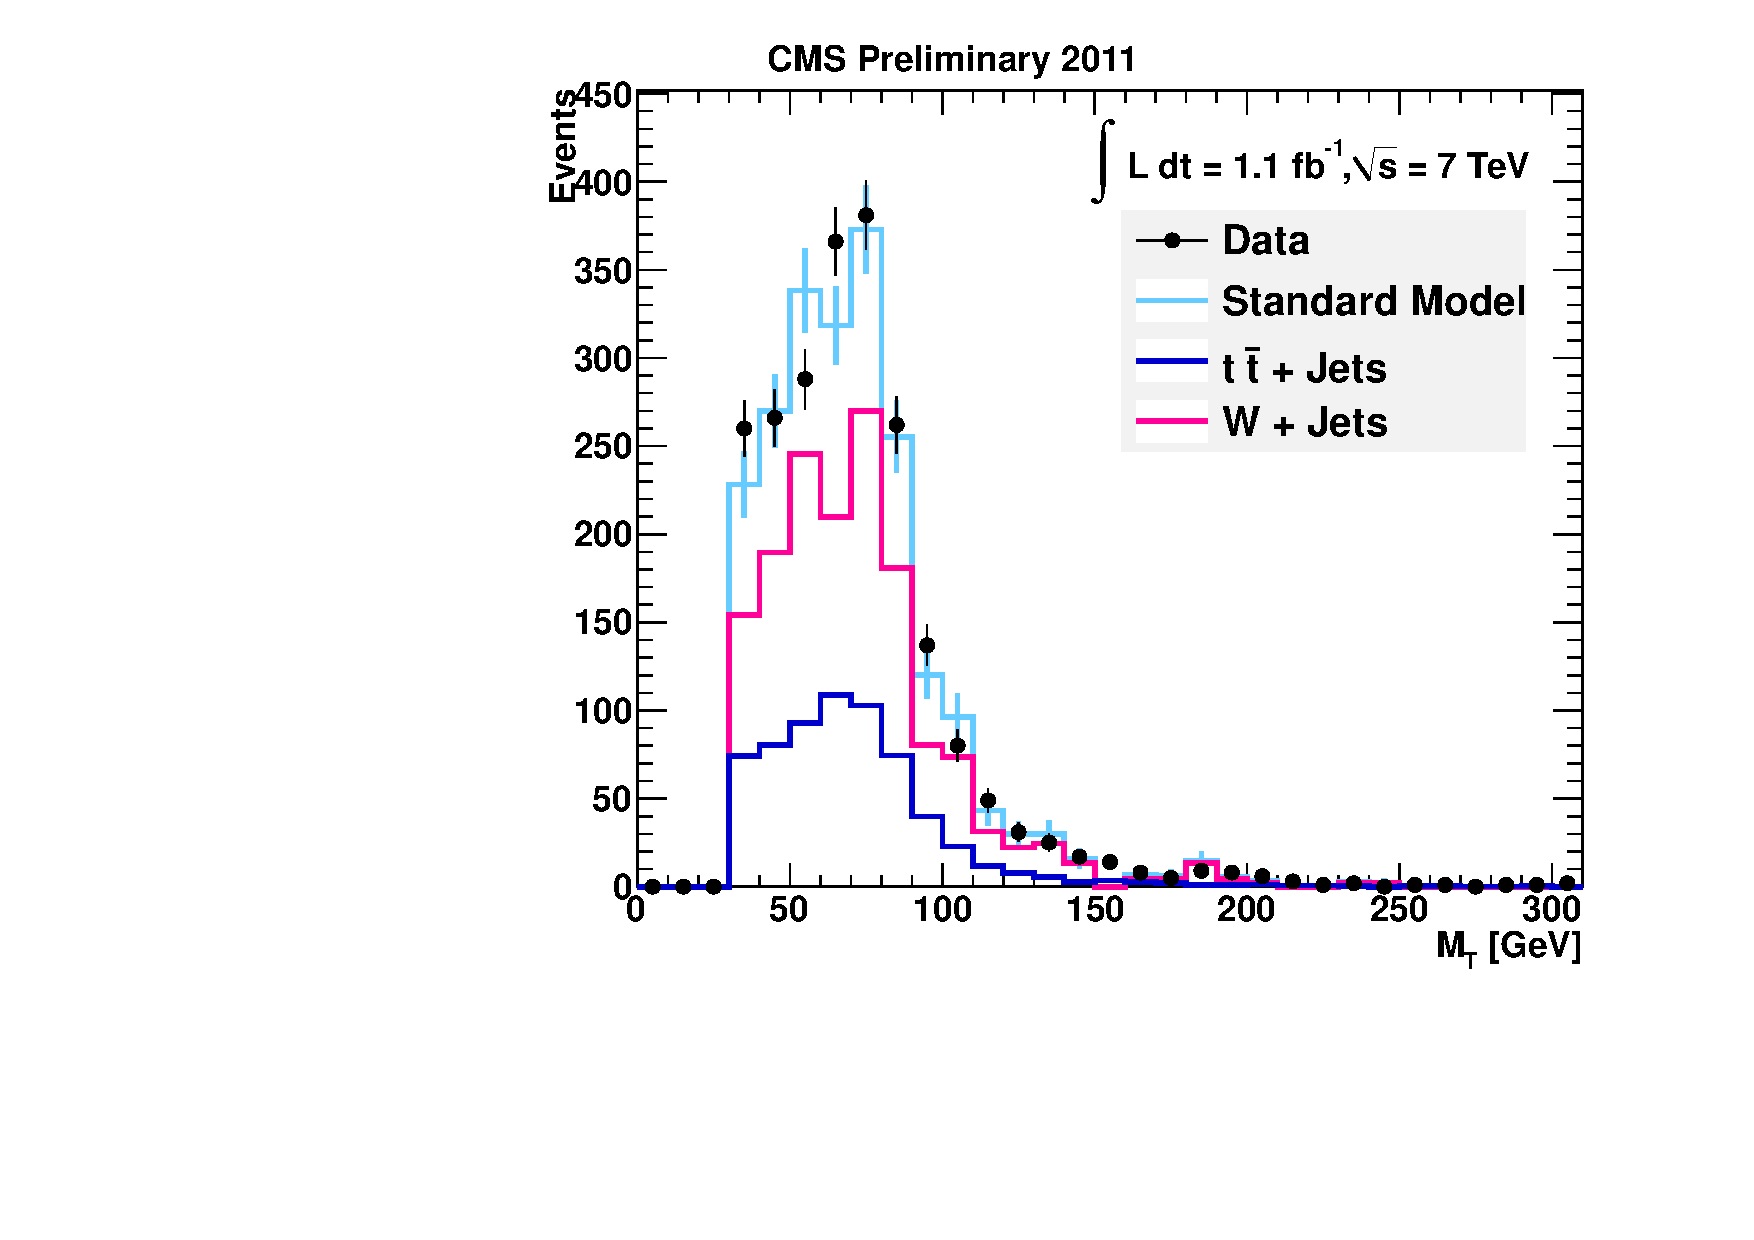
\includegraphics[width=0.45\textwidth, angle=0]{Figures/Analysis/PAS/muon_plots/spring11NoLogYMTMuonControl_beforeaT.pdf}}

\caption{\label{fig:muonplots_beforeat} Data - Monte Carlo comparisons
  for the muon control selection before the $\alpha_{T} > 0.55$ cut is
  applied, shown for (a) $\alpha_{T}$ and (b) $H_{T}$, (c) Muon  Combined Isolation and (d) $M_{T}$.
 A cut of $\mathrm{HT >}$375 GeV has been applied, to select the
 region of fixed jet thresholds.}
\label{fig:kin}
\end{center}
\end{figure}

\begin{figure}[h]
\begin{center}
\subfigure[\label{fig:muon_beforeat_mupt}]{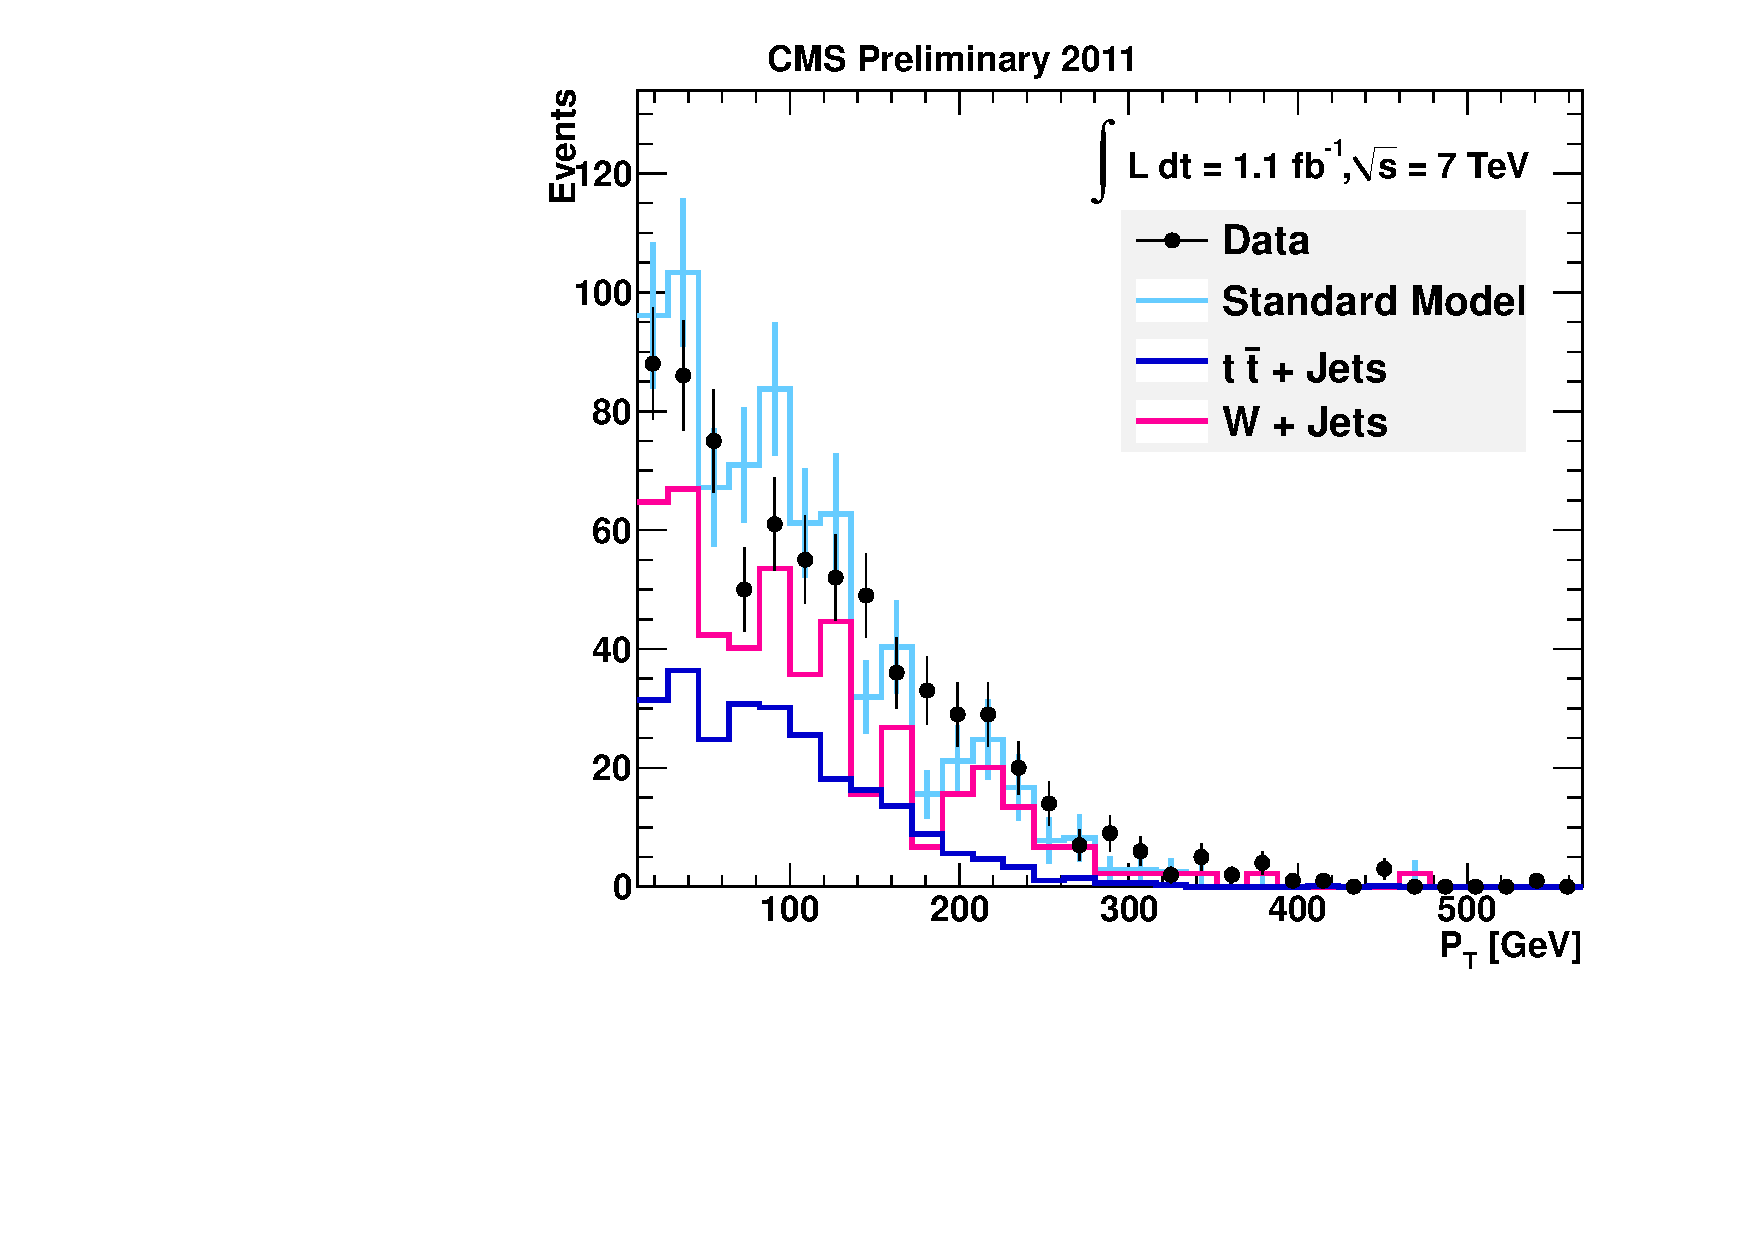
\includegraphics[width=0.45\textwidth, angle=0]{Figures/Analysis/PAS/muon_plots/spring11NoLogYMuPtMuonControl_afteraT.pdf}}
\subfigure[\label{fig:muon_beforeat_njet}]{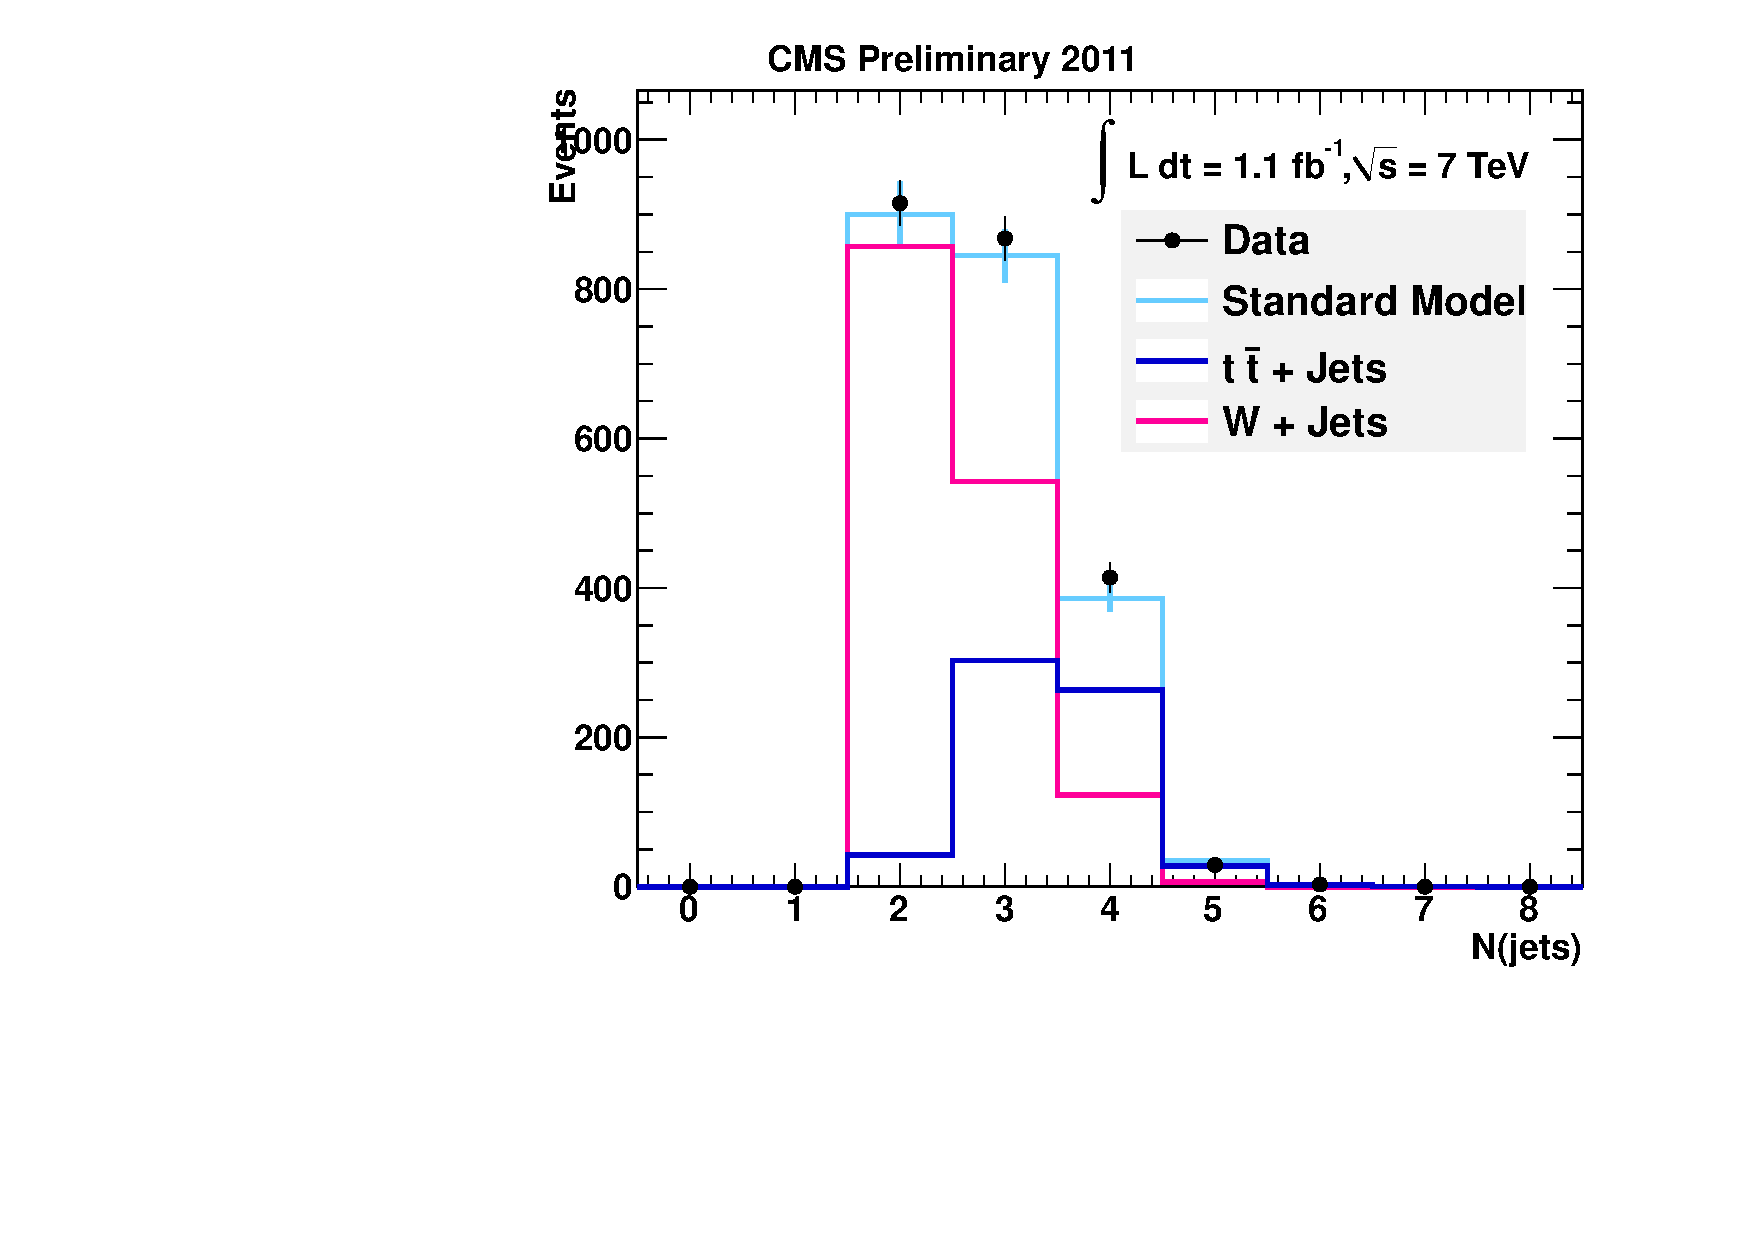
\includegraphics[width=0.45\textwidth, angle=0]{Figures/Analysis/PAS/muon_plots/spring11NoLogYnJetMuonControl_beforeaT.pdf}}
\newline

\subfigure[\label{fig:muon_afterat_at}]{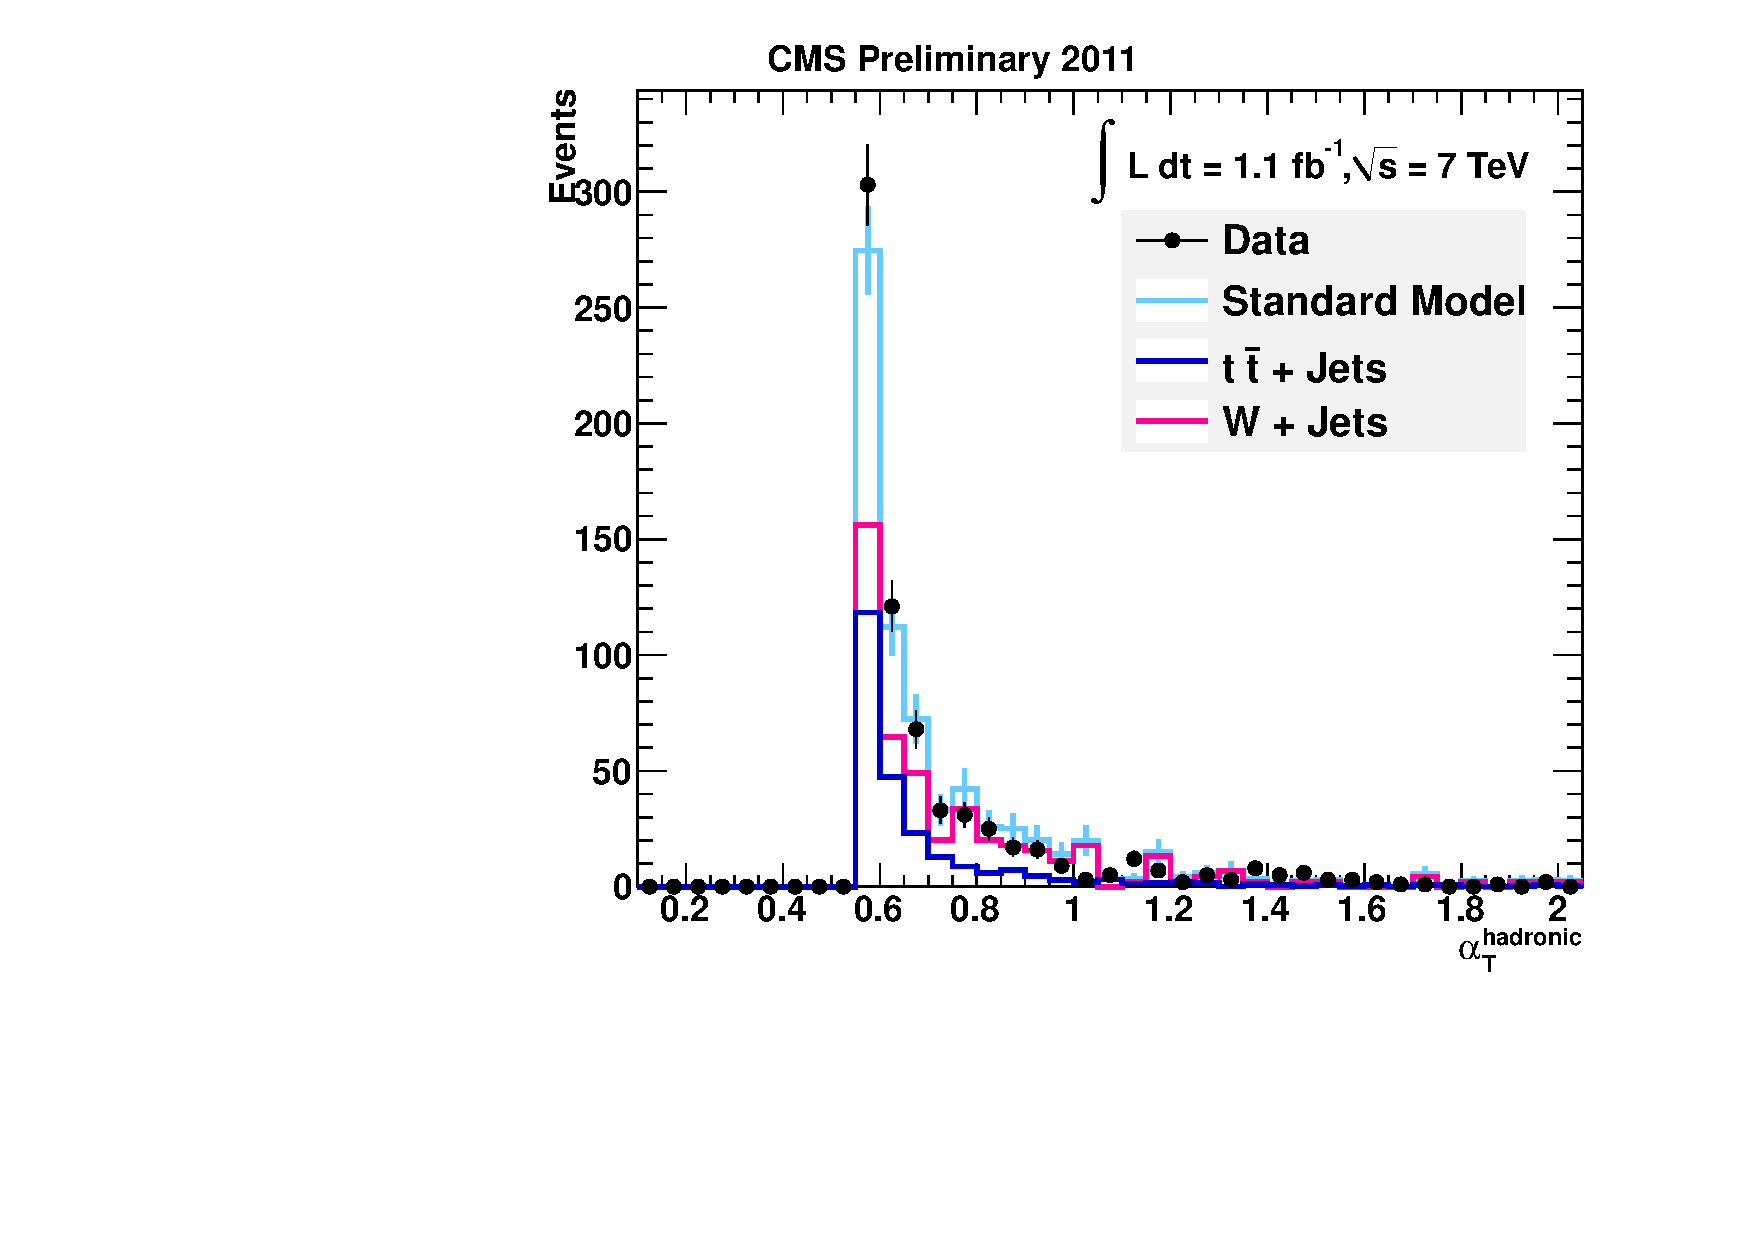
\includegraphics[width=0.45\textwidth, angle=0]{Figures/Analysis/PAS/muon_plots/spring11NoLogYaT_HMuonControl_afteraT.pdf}}
\subfigure[\label{fig:muon_afterat_ht}]{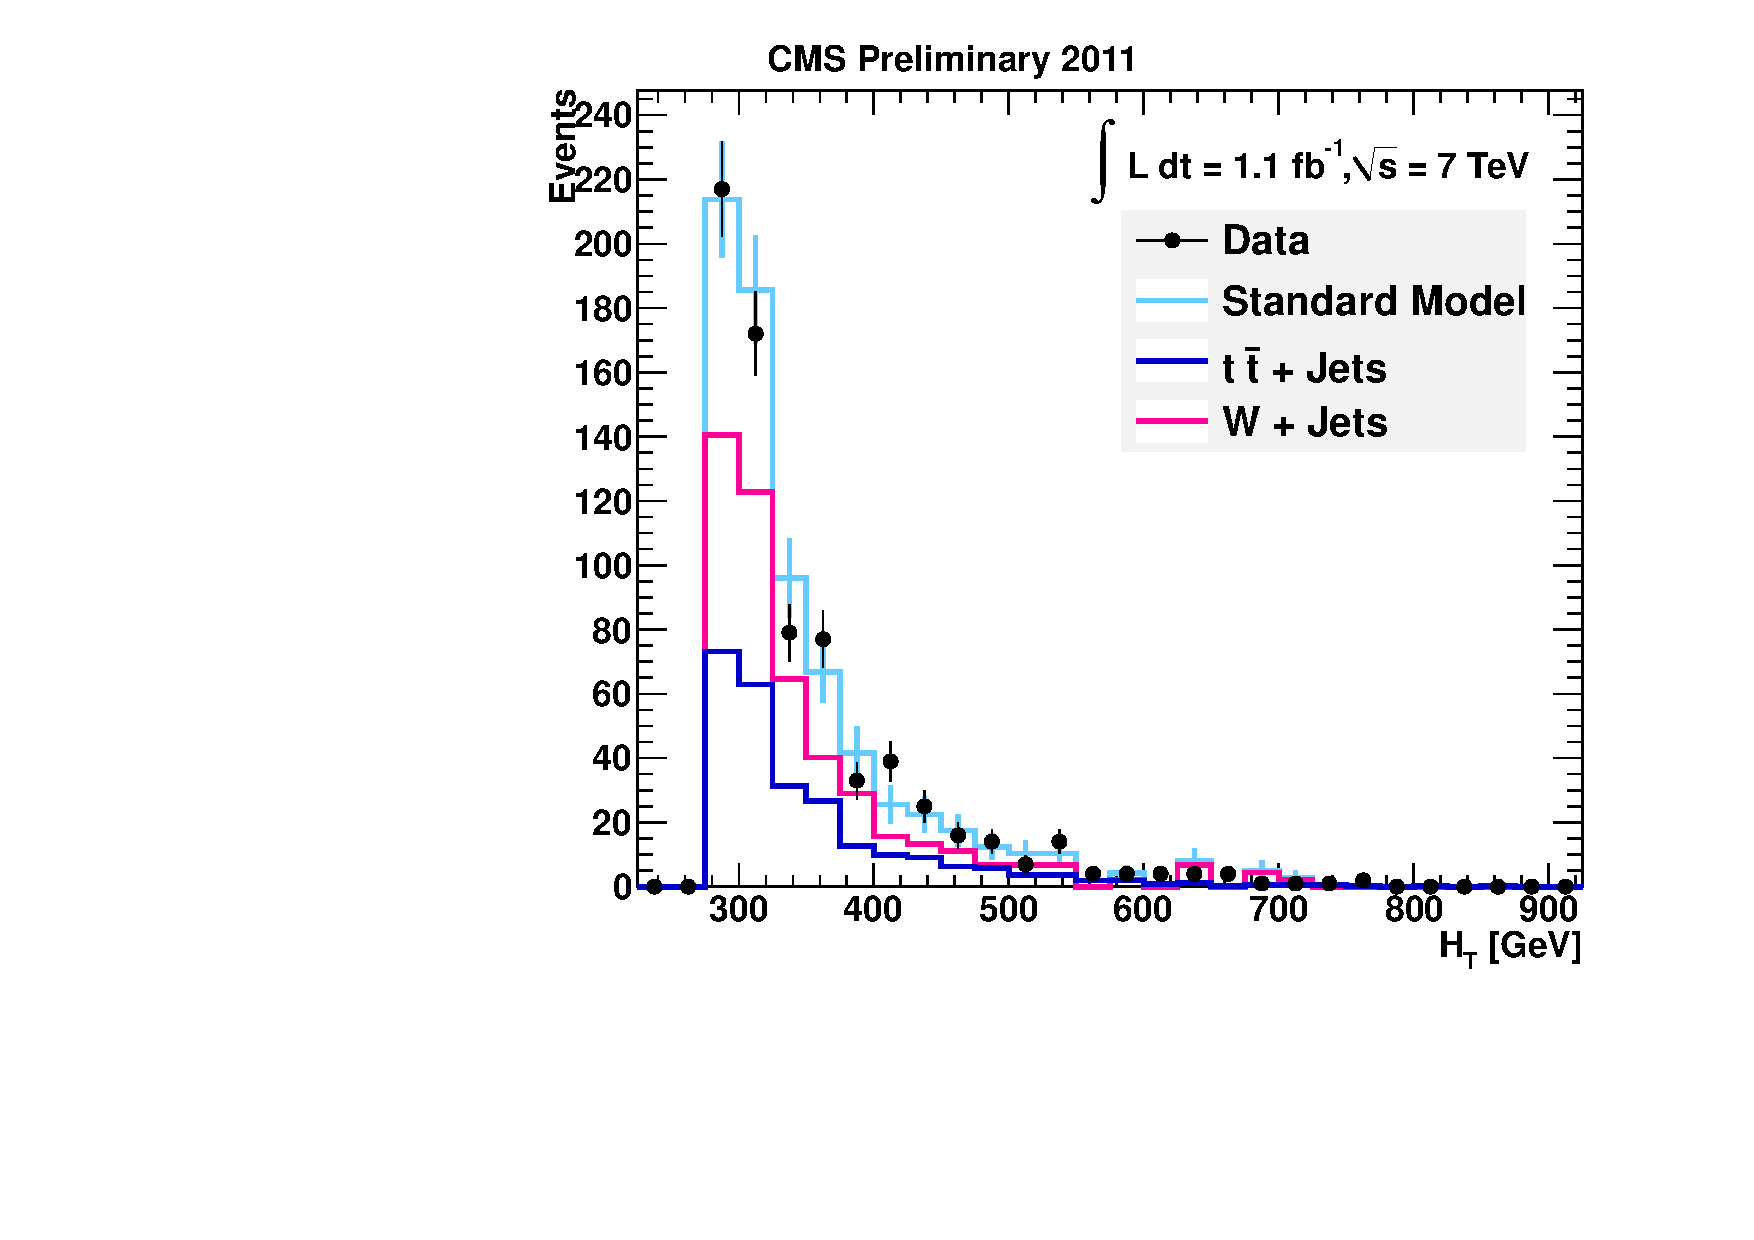
\includegraphics[width=0.45\textwidth, angle=0]{Figures/Analysis/PAS/muon_plots/spring11NoLogYHTMuonControl_afteraT.pdf}}
\newline
\subfigure[\label{fig:muon_afterat_MuIso}]{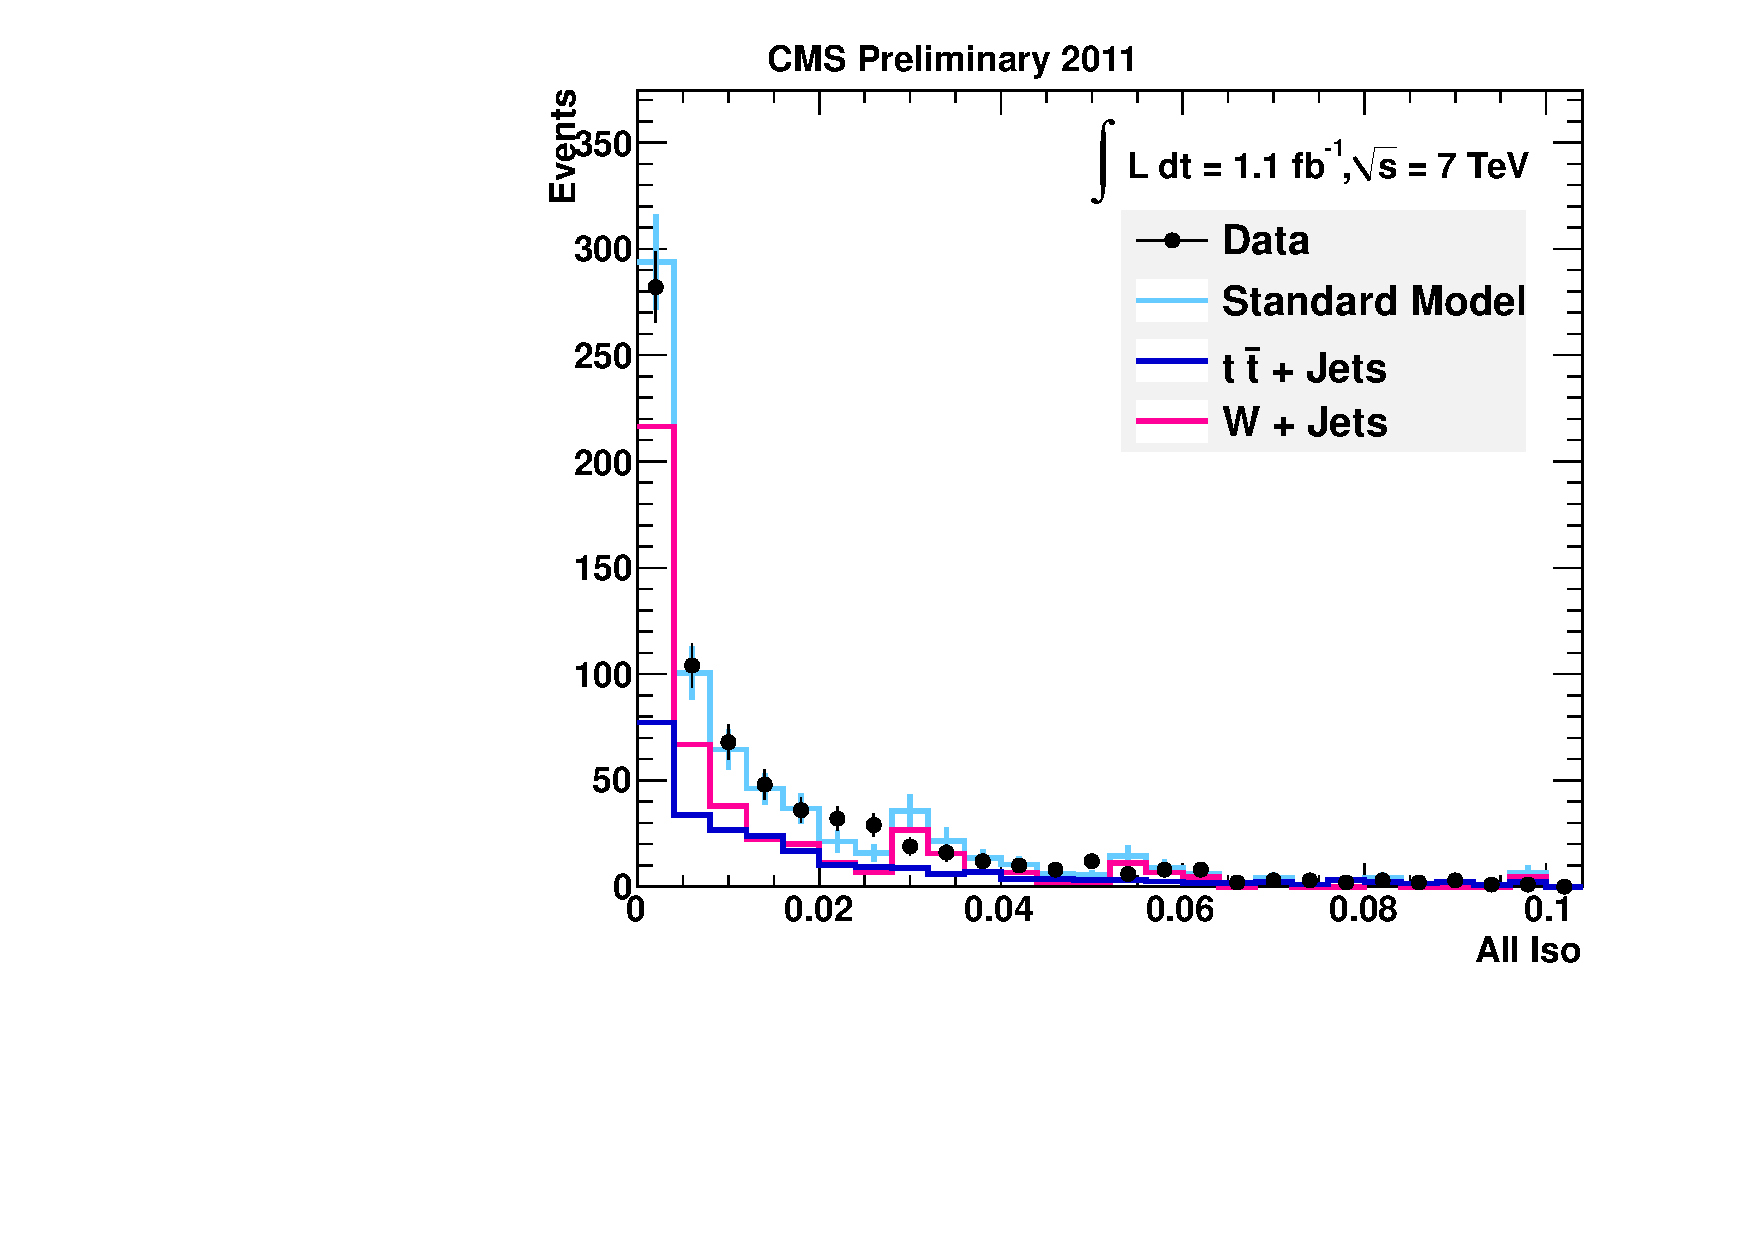
\includegraphics[width=0.45\textwidth, angle=0]{Figures/Analysis/PAS/muon_plots/spring11NoLogYMuCsoMuonControl_afteraT.pdf}}
\subfigure[\label{fig:muon_afterat_mt}]{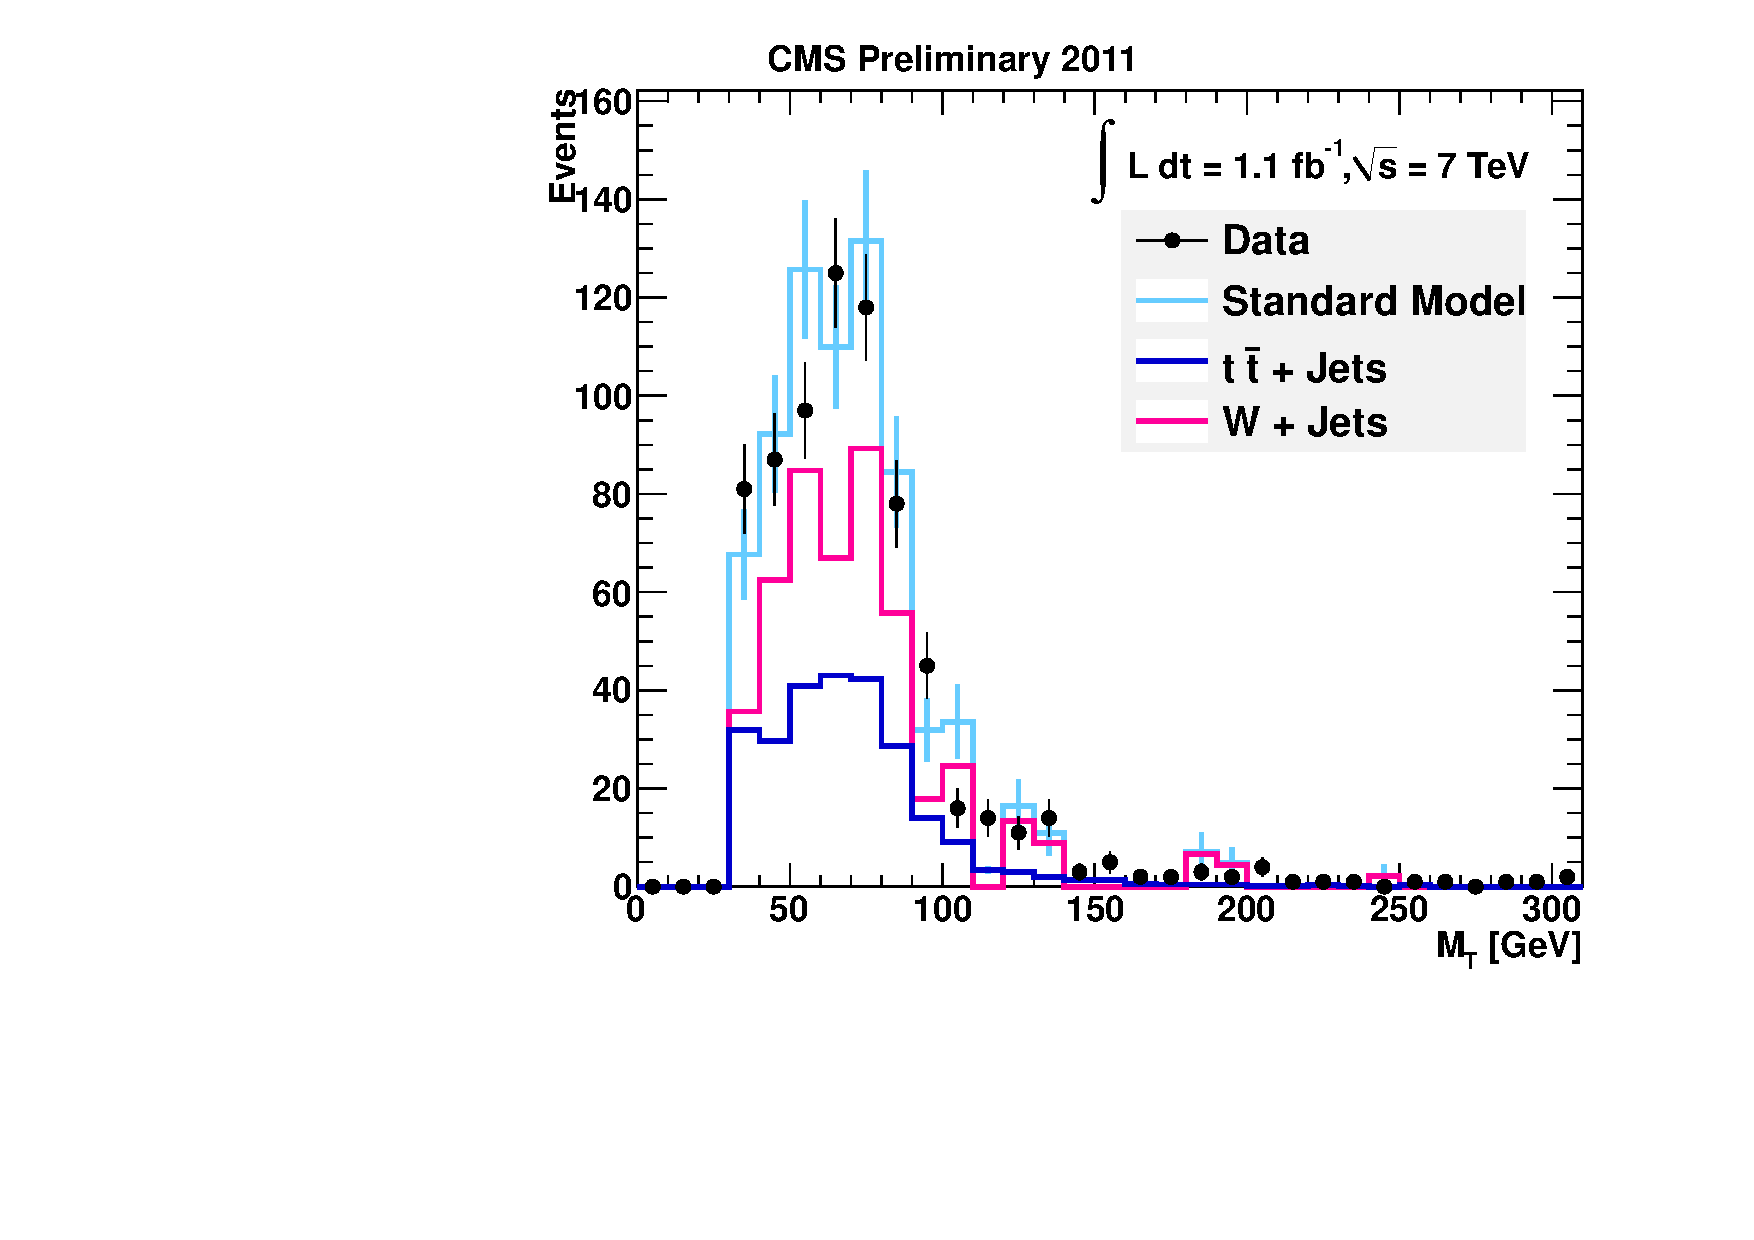
\includegraphics[width=0.45\textwidth, angle=0]{Figures/Analysis/PAS/muon_plots/spring11NoLogYMTMuonControl_afteraT.pdf}}

\caption{\label{fig:muonplots_afterat} Data - Monte Carlo comparisons
  for the muon control selection after the $\alpha_{T} > 0.55$ cut is
  applied, shown for (a) \scalht and (b) $M_T$, (c) Muon  Combined Isolation and (d) $M_{T}$.
 A cut of $\mathrm{HT >}$375 GeV has been applied, to select the
 region of fixed jet thresholds.}
\label{fig:kin}
\end{center}
\end{figure}

\subsubsection{Types of decay contributing to Muon Control Sample}

\begin{figure}[h]
\begin{center}
\subfigure[\label{fig:muon_types_275TT}]{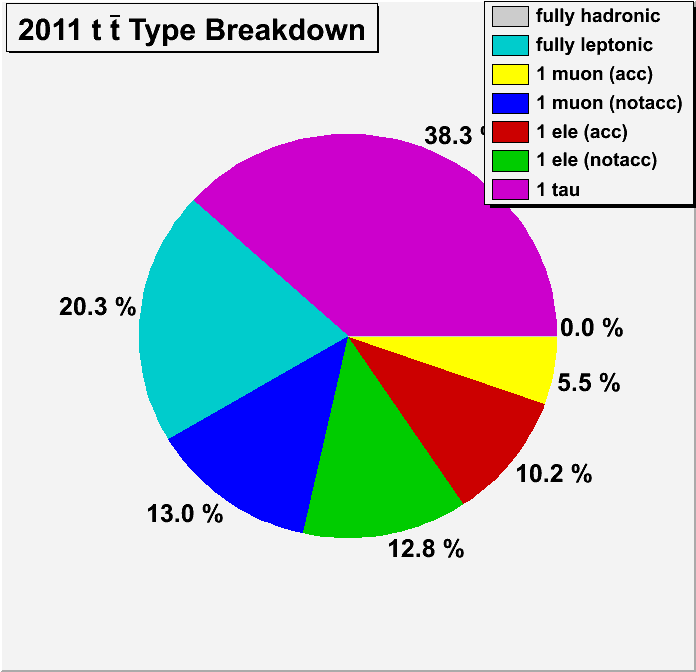
\includegraphics[width=0.40\textwidth, angle=0]{Figures/Analysis/Types/2011_275_TT_Pie}}
\subfigure[\label{fig:muon_types_275W}] {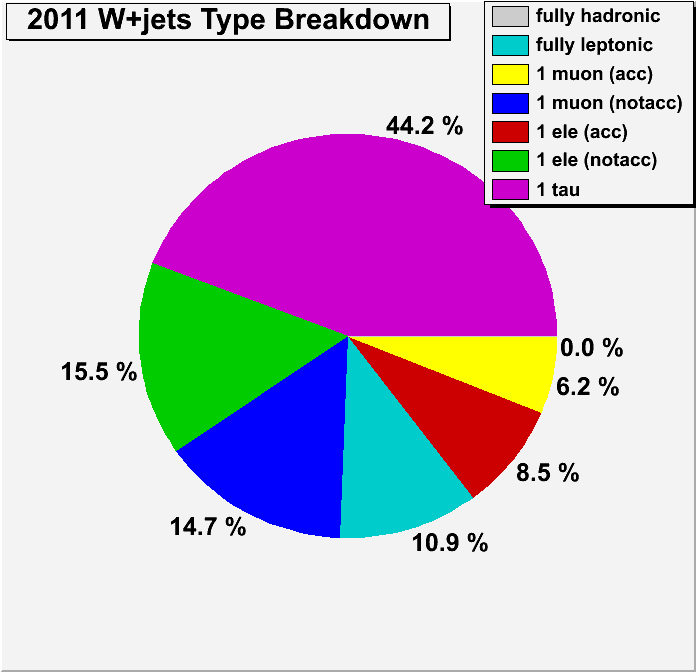
\includegraphics[width=0.40\textwidth, angle=0]{Figures/Analysis/Types/2011_275_W_Pie}}
\newline
\subfigure[\label{fig:muon_types_325TT}]{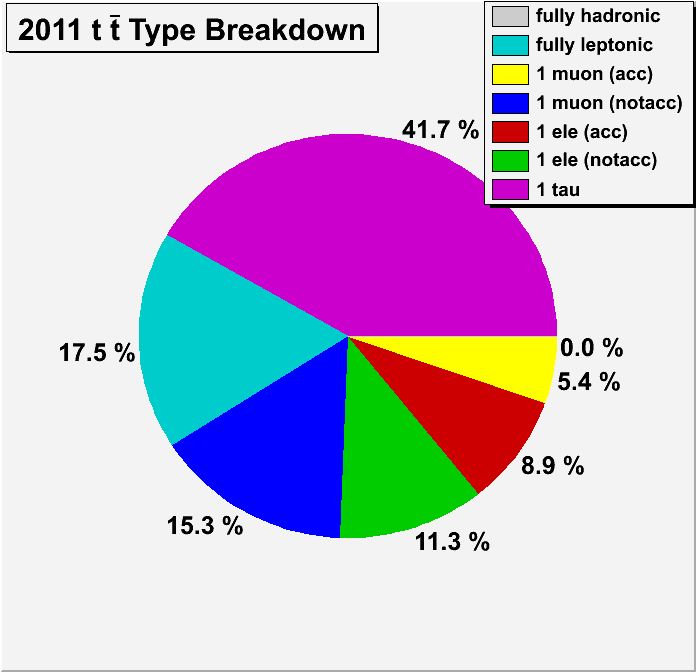
\includegraphics[width=0.40\textwidth, angle=0]{Figures/Analysis/Types/2011_325_TT_Pie}}
\subfigure[\label{fig:muon_types_325W}] {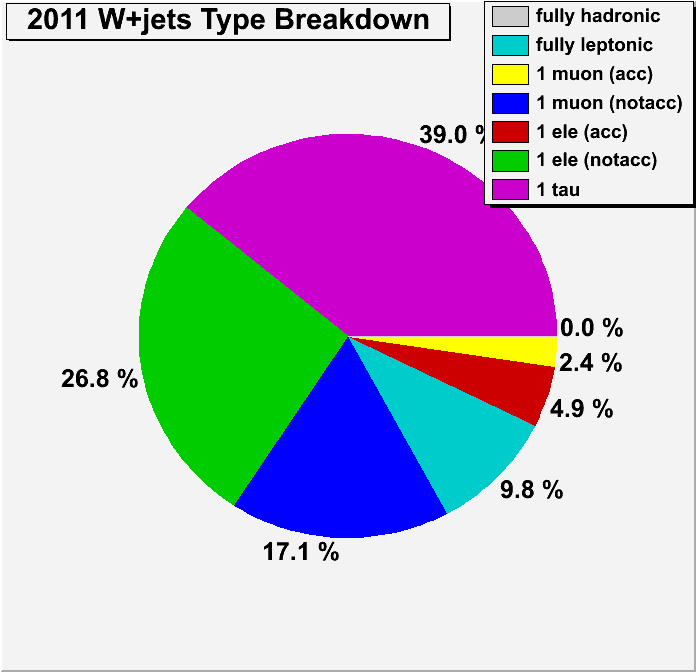
\includegraphics[width=0.40\textwidth, angle=0]{Figures/Analysis/Types/2011_325_W_Pie}}
\newline
\subfigure[\label{fig:muon_types_allTT}]{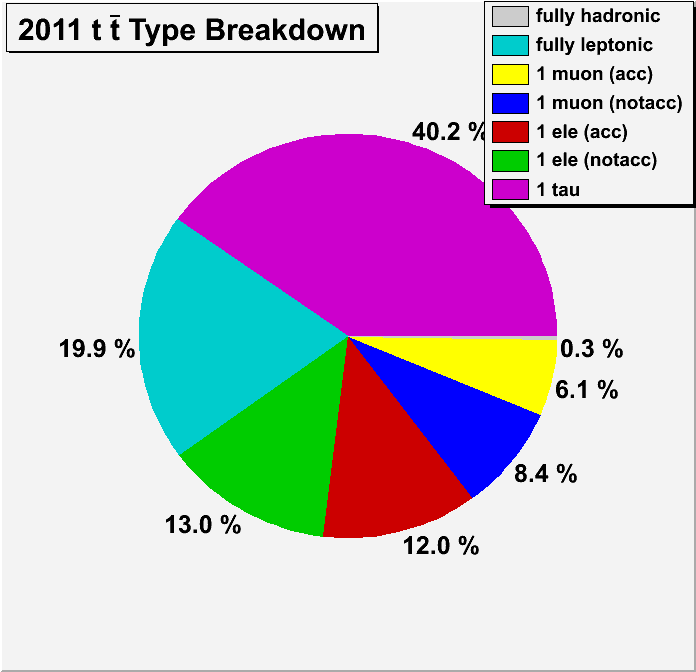
\includegraphics[width=0.40\textwidth, angle=0]{Figures/Analysis/Types/2011_unsca375_TT_Pie}}
\subfigure[\label{fig:muon_types_allW}] {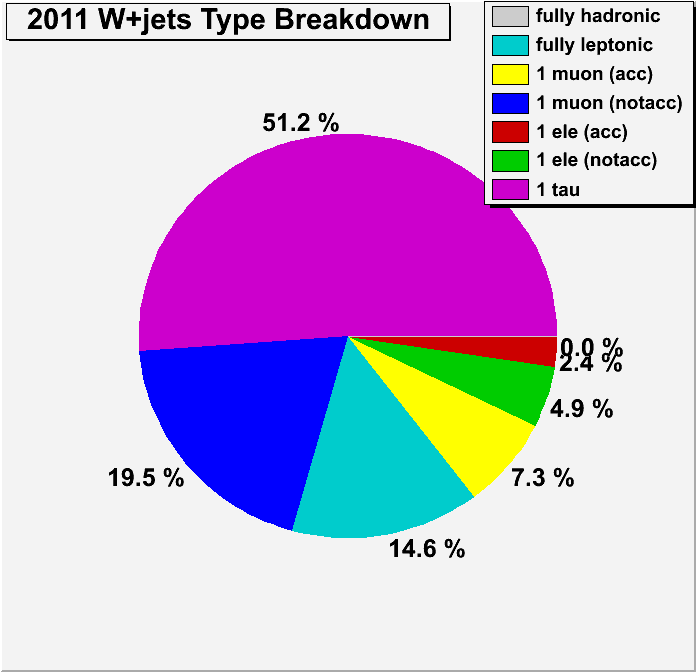
\includegraphics[width=0.40\textwidth, angle=0]{Figures/Analysis/Types/2011_unsca375_W_Pie}}

\caption{\label{fig:muon_types} Type breakdown of decays resulting in an event selected by the Muon Control selection, shown using Monte-Carlo truth information separately for \ttj (left) and \wj (right) events. The breakdown is made separately for each jet-scale case: 275 \less \HT \less 325 GeV (top), 325 \less \HT \less 375 GeV (middle), and \HT \more 375 GeV (bottom). }
\end{center}
\end{figure}

\subsection{Estimation Z  $\nu \bar{\nu}$ + jets background using photon + jets events}

\begin{figure}[h]
\begin{center}
\subfigure[\label{fig:photon_alphaT}]{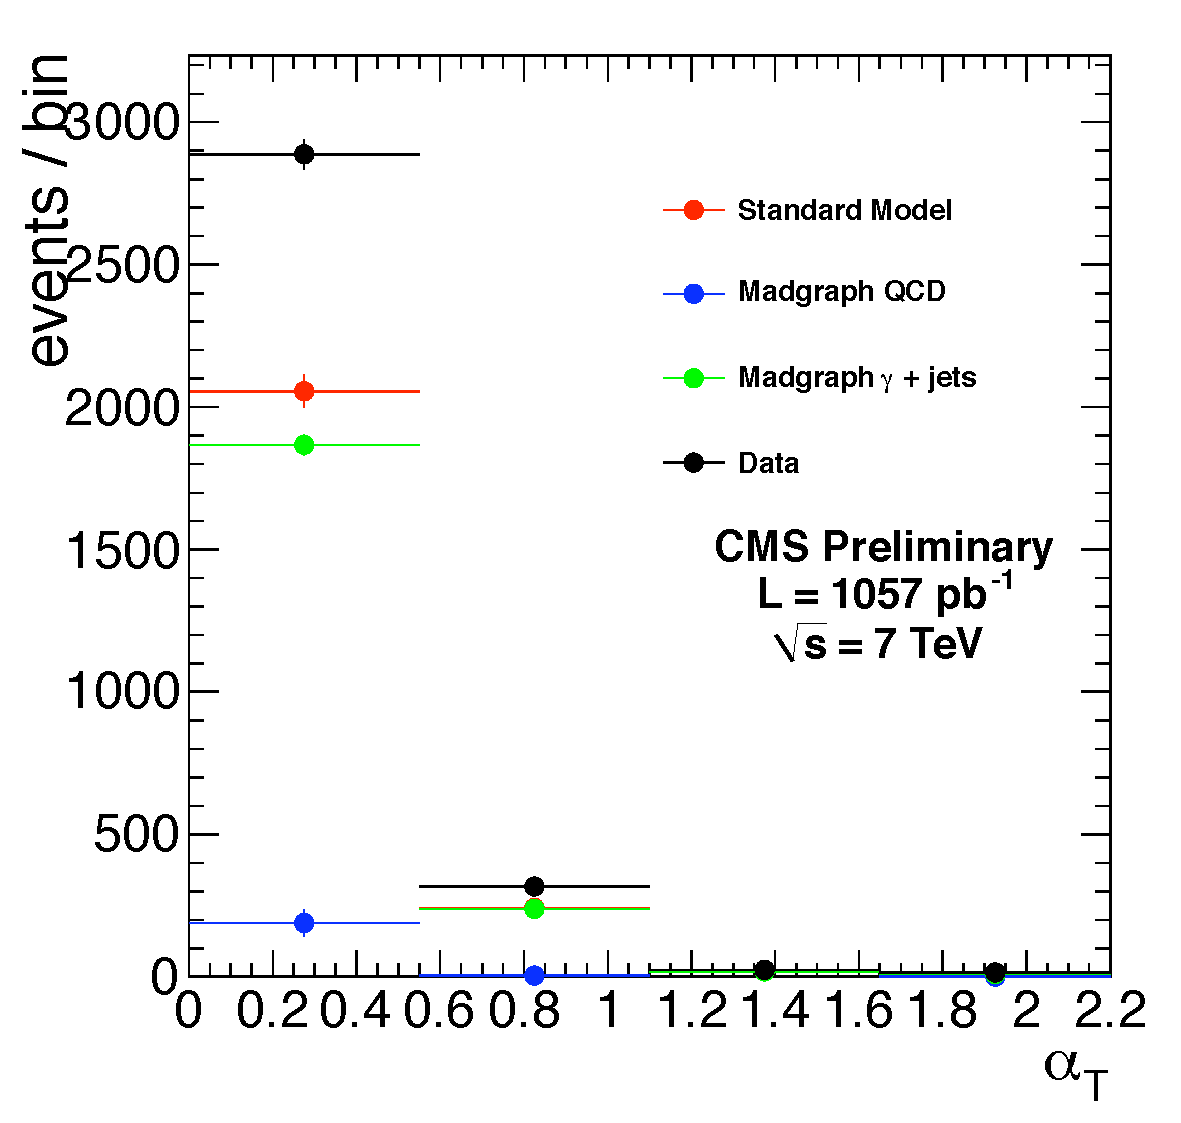
\includegraphics[width=0.45\textwidth, angle=0]{Figures/Analysis/PAS/photon_plots/375___xcak5JetAlphaTFewBinsPat.pdf}}
\subfigure[\label{fig:photon_nJets}] {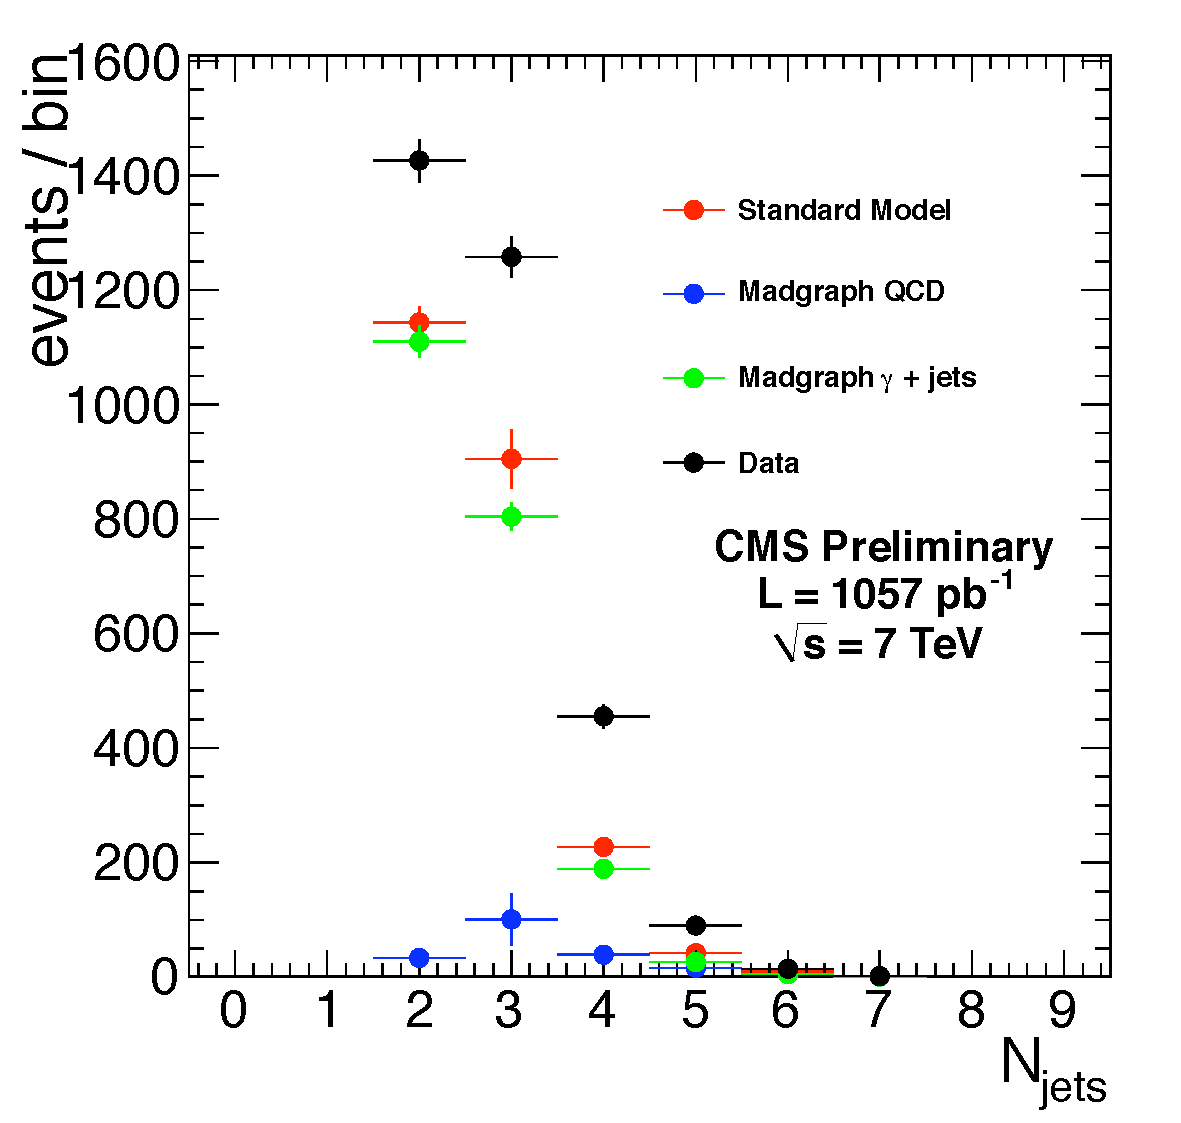
\includegraphics[width=0.45\textwidth, angle=0]{Figures/Analysis/PAS/photon_plots/375___xcak5JetIndicesPat.pdf}}
\caption{\label{fig:photon_plots} Data-MC comparisons for the photon control sample.  $\scalht > 375$~GeV and $\mht/\scalht>0.4$ are required.   Left: the distribution of $\alpha_{T}$.  Right: the distribution of the number of jets.}
\end{center}
\end{figure}

\section{Systematic Uncertainties}
\section{Simultaneous Fit}


 \begin{figure}[h]
   \begin{center}
     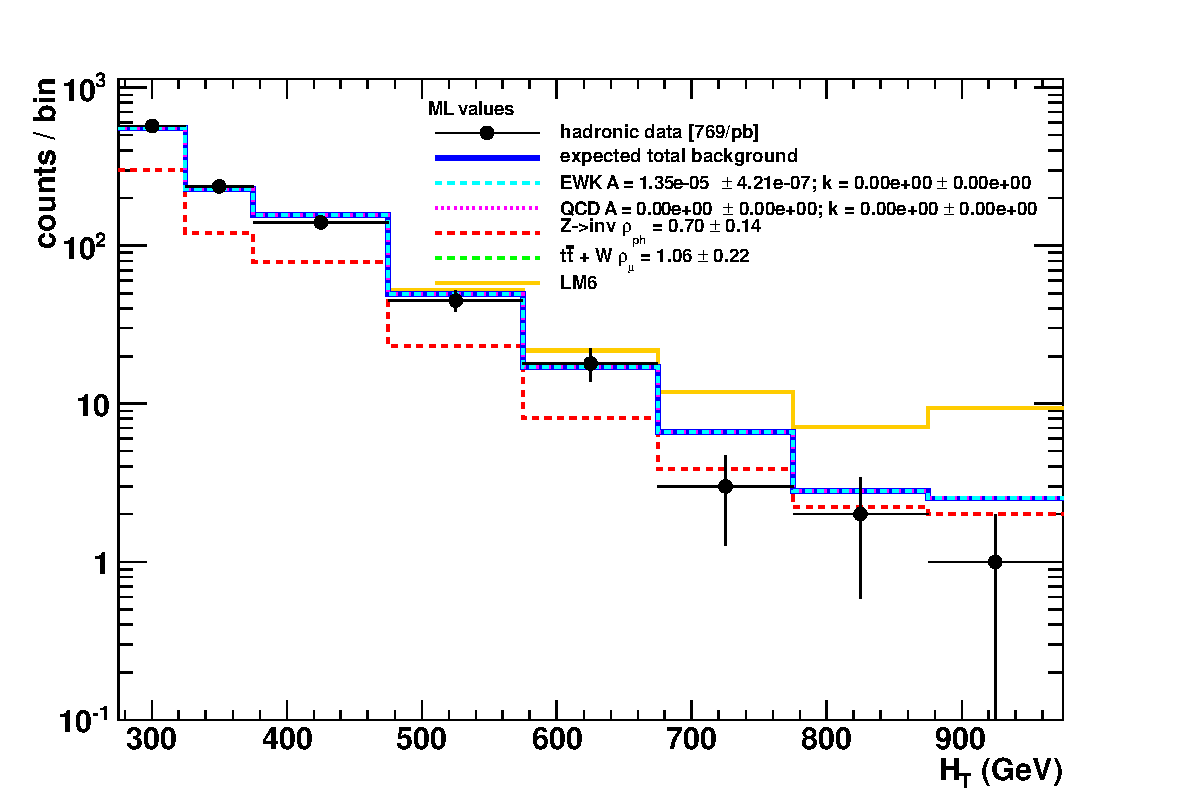
\includegraphics[width = 0.48\textwidth]{Figures/Analysis/PAS/stats_plots/RQcdZero/hadronic_signal_fit_logy.pdf}
     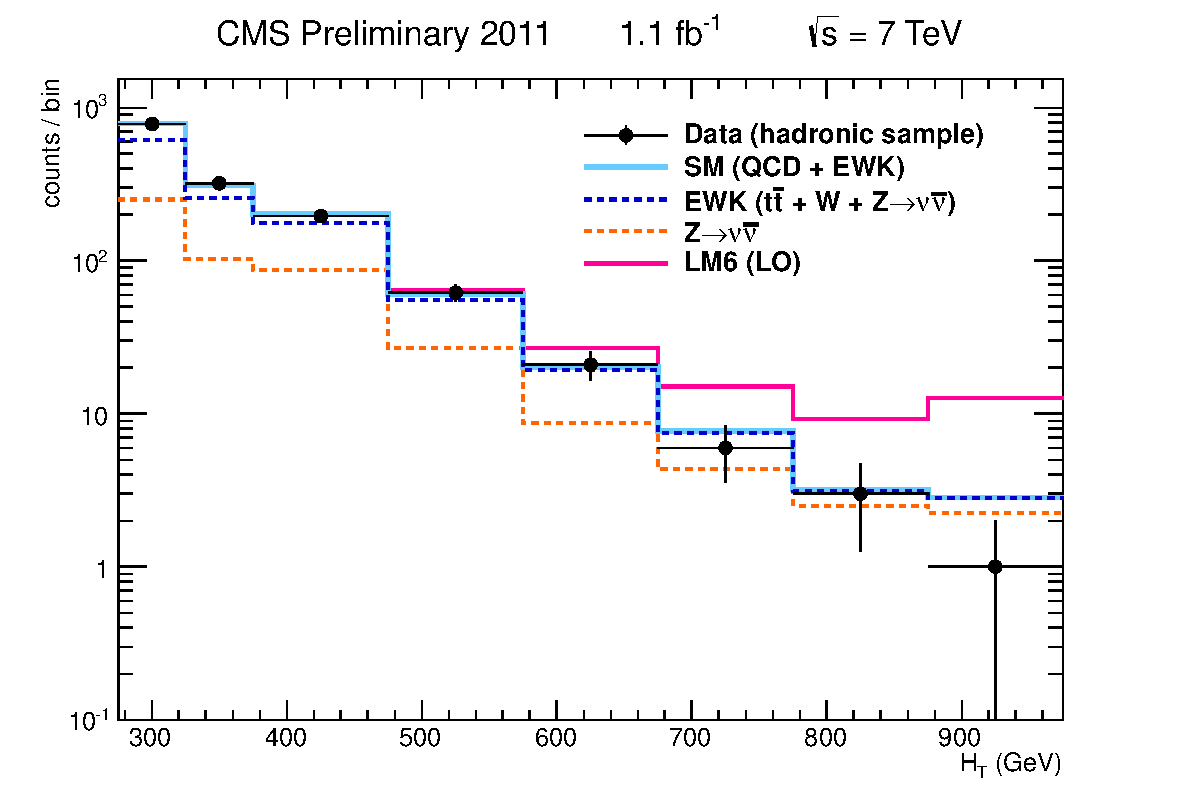
\includegraphics[width = 0.48\textwidth]{Figures/Analysis/PAS/stats_plots/RQcdFallingExp/hadronic_signal_fit_logy.pdf}
     \caption{\label{fig:hadronic} \scalht distribution for events in the hadronic signal sample for scenario a) (left) and scenario b) (right). Shown are the events observed in data (black points), the outcome of the fit (blue line) and a breakdown of the individual background contributions as predicted by the control samples. A possible signal contribution from benchmark point LM6 is indicated as well (yellow line).}
   \end{center}
 \end{figure}

 \begin{figure}[h]
   \begin{center}
     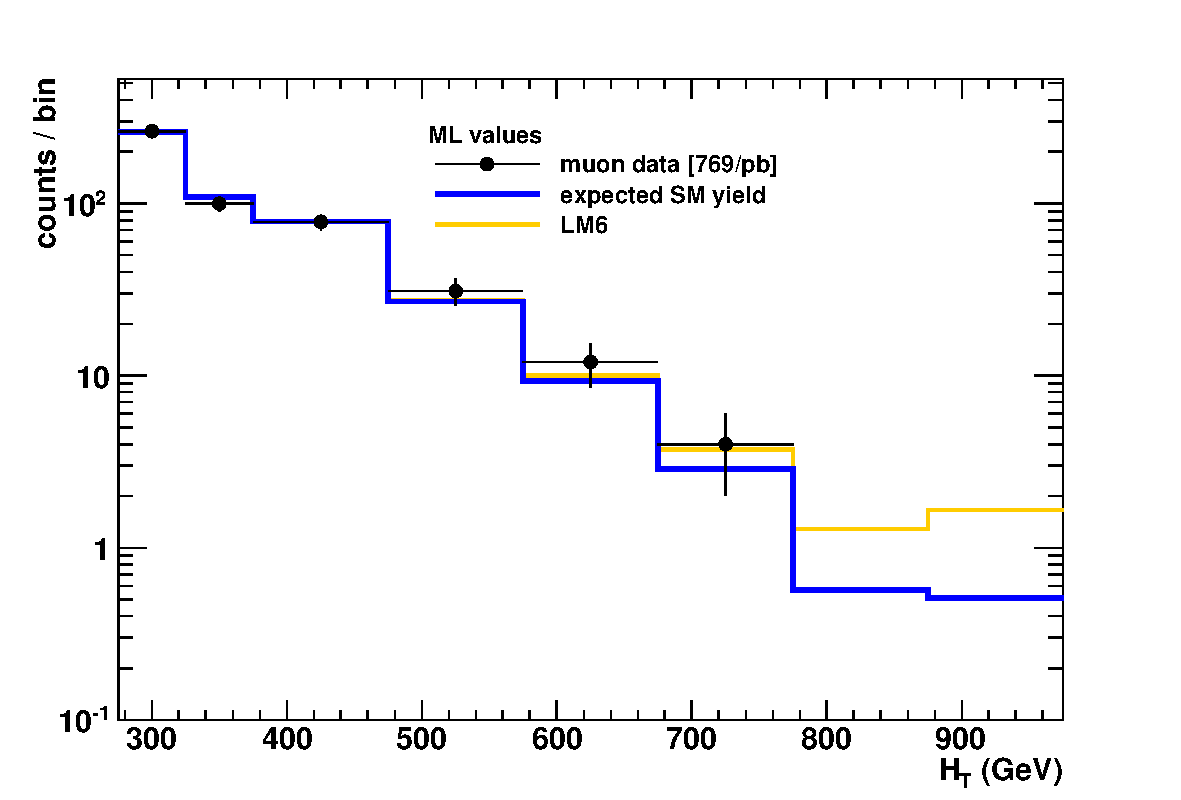
\includegraphics[width = 0.48\textwidth]{Figures/Analysis/PAS/stats_plots/RQcdZero/muon_control_fit_logy.pdf}
     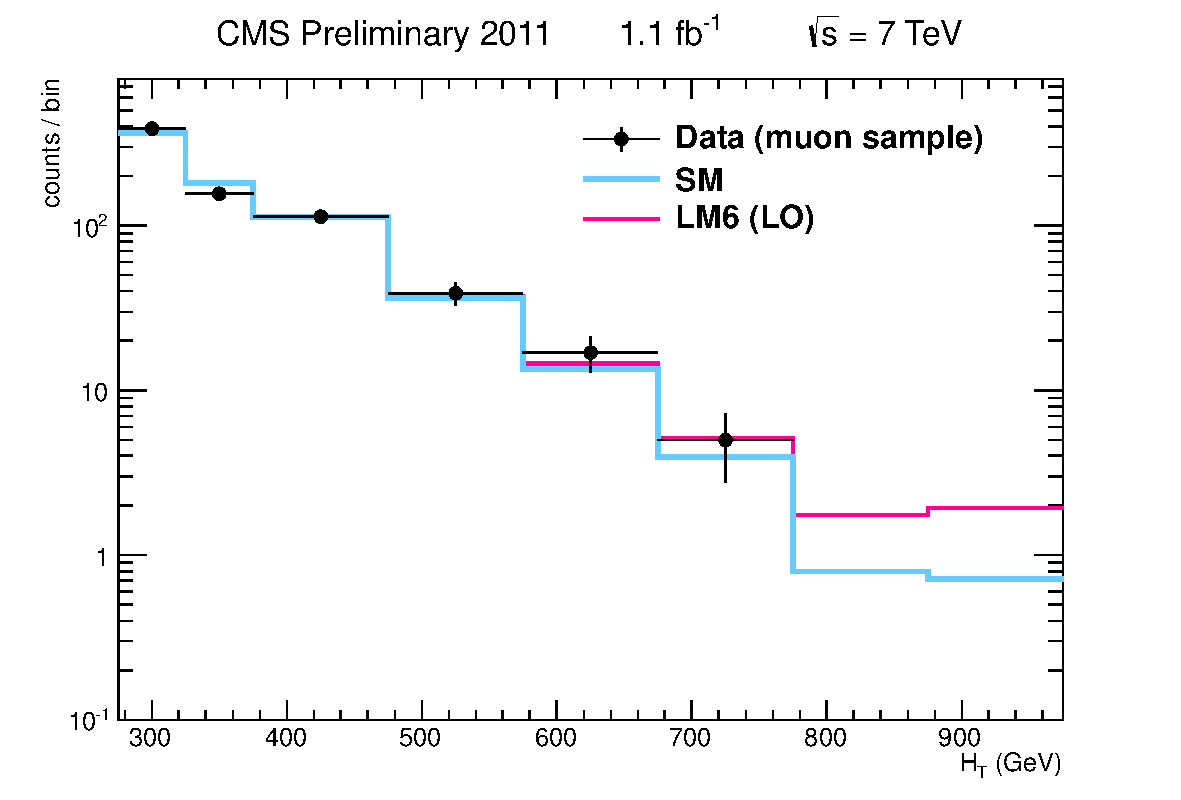
\includegraphics[width = 0.48\textwidth]{Figures/Analysis/PAS/stats_plots/RQcdFallingExp/muon_control_fit_logy.pdf}
     \caption{\label{fig:muon}  \scalht distribution for events selected in the muon control sample for scenario a) (left) and scenario b) (right).
  Shown are the events observed in data (black points), the outcome of the fit (blue line) and the MC expectation (dashed line). A possible signal
 contribution from benchmark point LM6 is indicated as well (yellow line).}
   \end{center}
 \end{figure}

 \begin{figure}[h]
   \begin{center}
     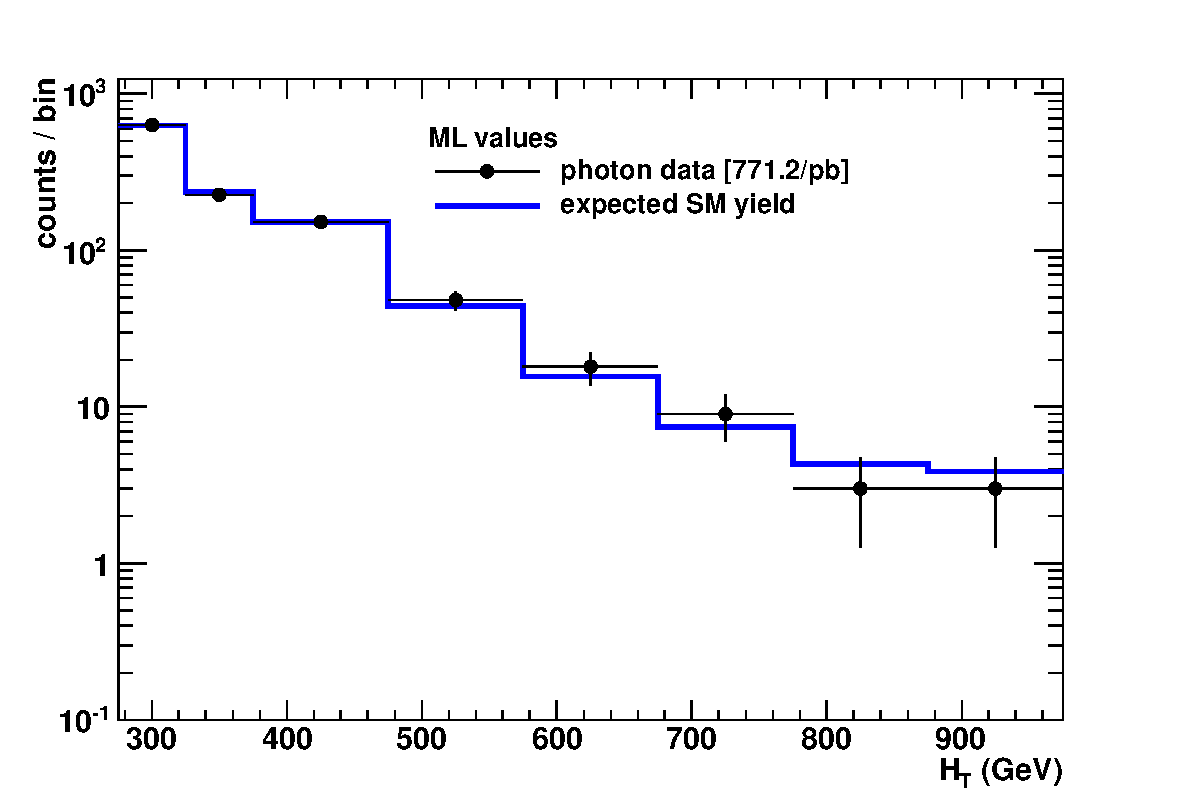
\includegraphics[width = 0.48\textwidth]{Figures/Analysis/PAS/stats_plots/RQcdZero/photon_control_fit_logy.pdf}
     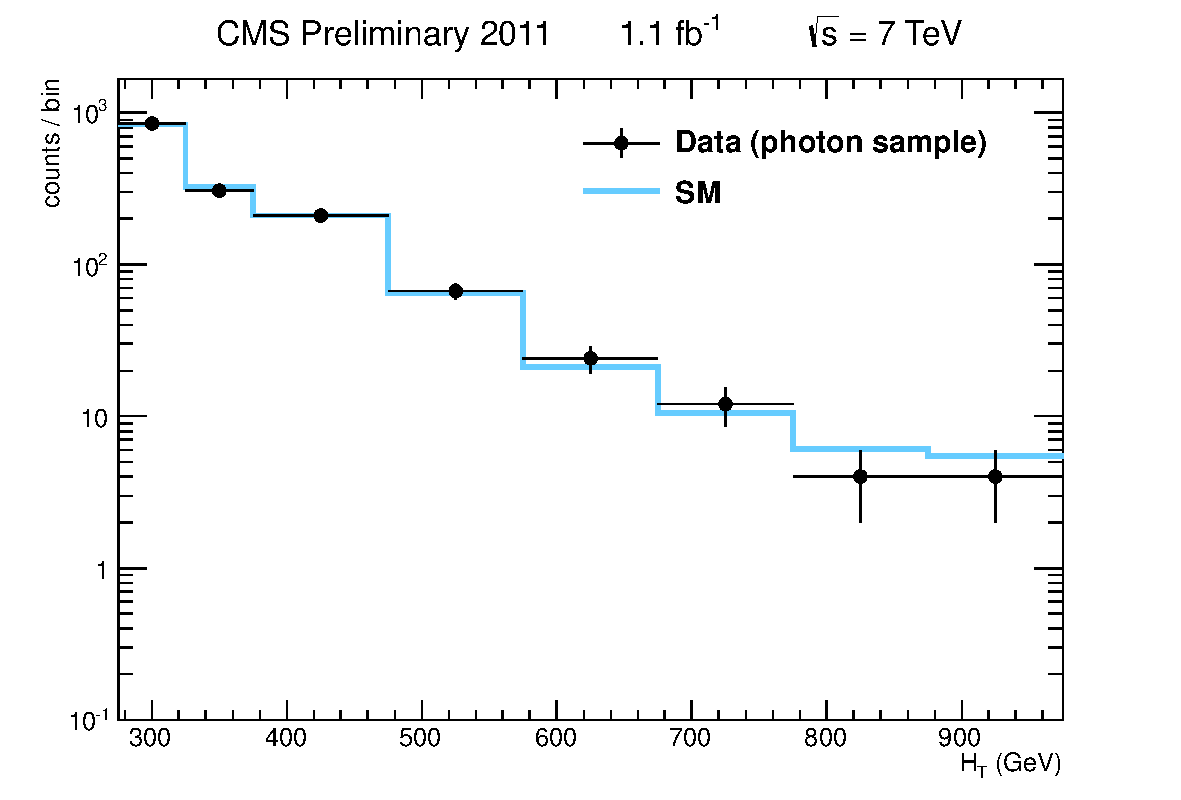
\includegraphics[width = 0.48\textwidth]{Figures/Analysis/PAS/stats_plots/RQcdFallingExp/photon_control_fit_logy.pdf}
     \caption{\label{fig:photon} \scalht distribution for events selected in the photon control sample for scenario a) (left) and scenario b) (right). Shown are the events observed in data (black points), the outcome of the fit (blue line) and the MC expectation (dashed line).}
   \end{center}
 \end{figure}

 \begin{figure}[h]
   \begin{center}
     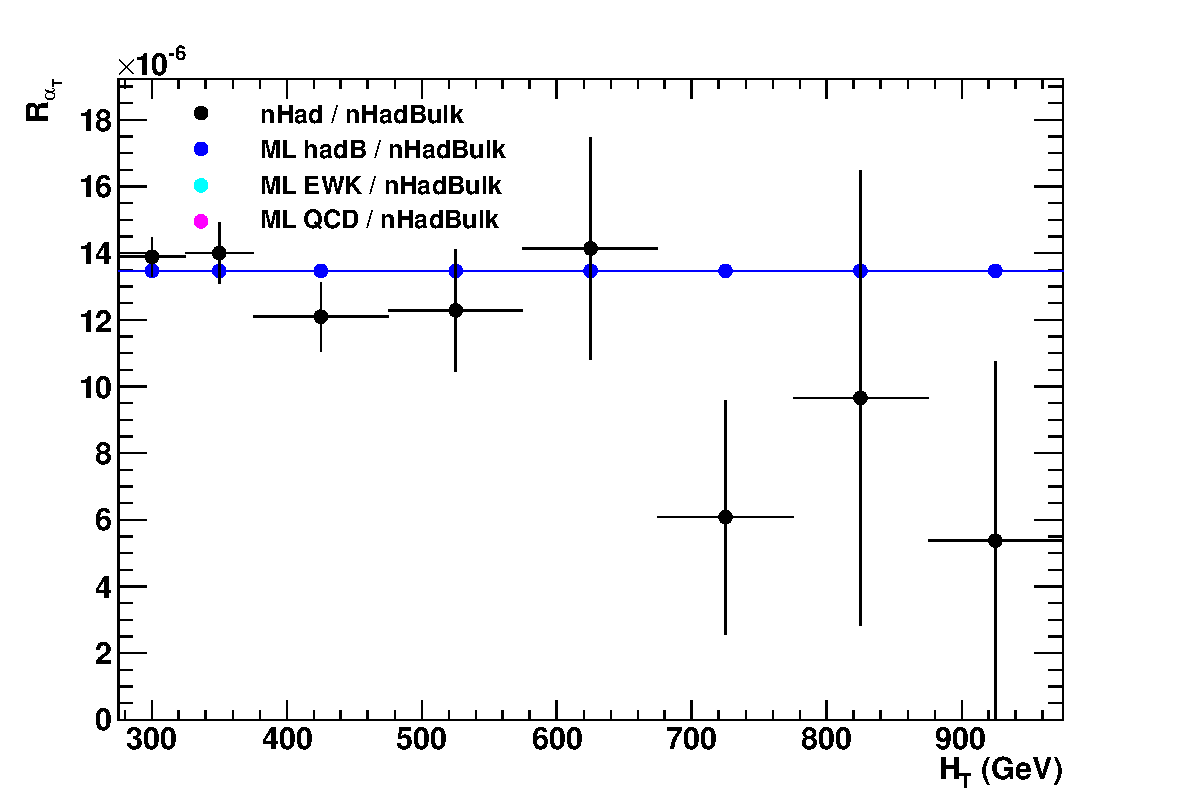
\includegraphics[width = 0.48\textwidth]{Figures/Analysis/PAS/stats_plots/RQcdZero/hadronic_signal_alphaT_ratio.pdf}
     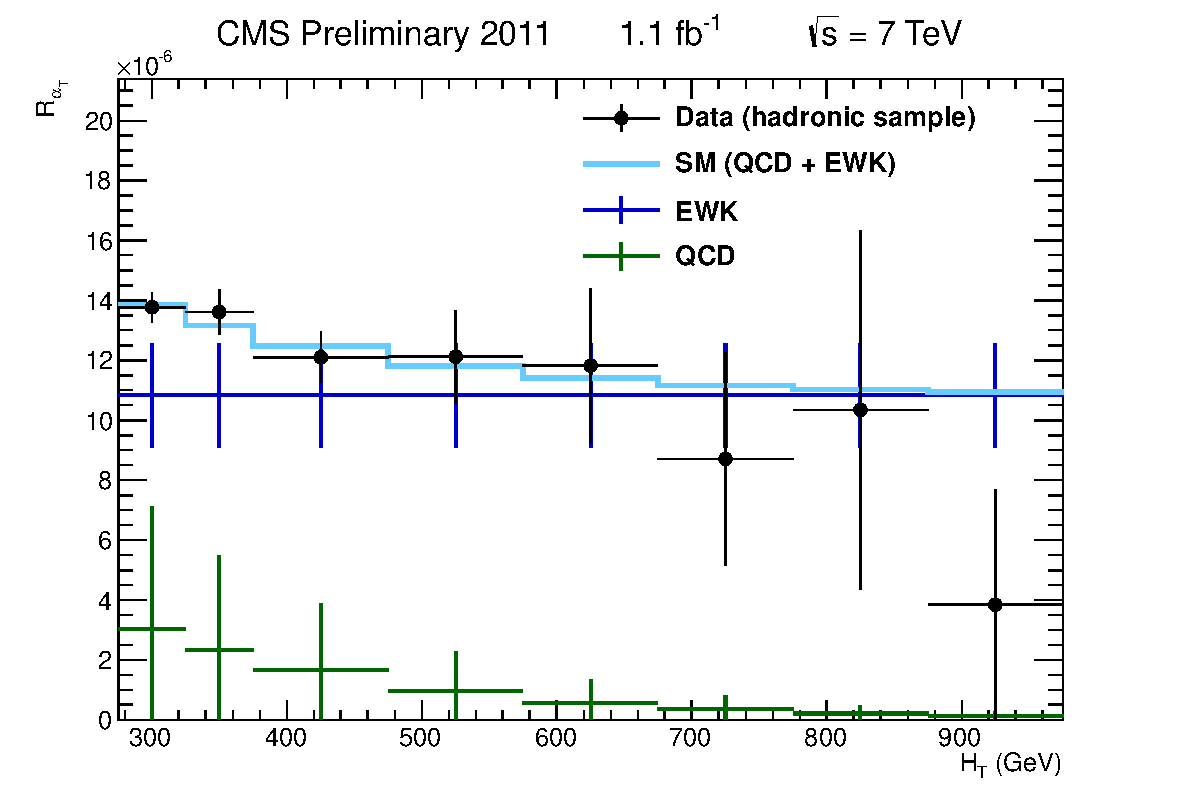
\includegraphics[width = 0.48\textwidth]{Figures/Analysis/PAS/stats_plots/RQcdFallingExp/hadronic_signal_alphaT_ratio.pdf}
     \caption{\label{fig:rat} \RaT as a function of \scalht as observed in data (black points) and the results of the fit assuming different scenarios: a) (left) and b) (right) .}
   \end{center}
 \end{figure}

\section{Limits}

\begin{figure}[h]
  \begin{center}
    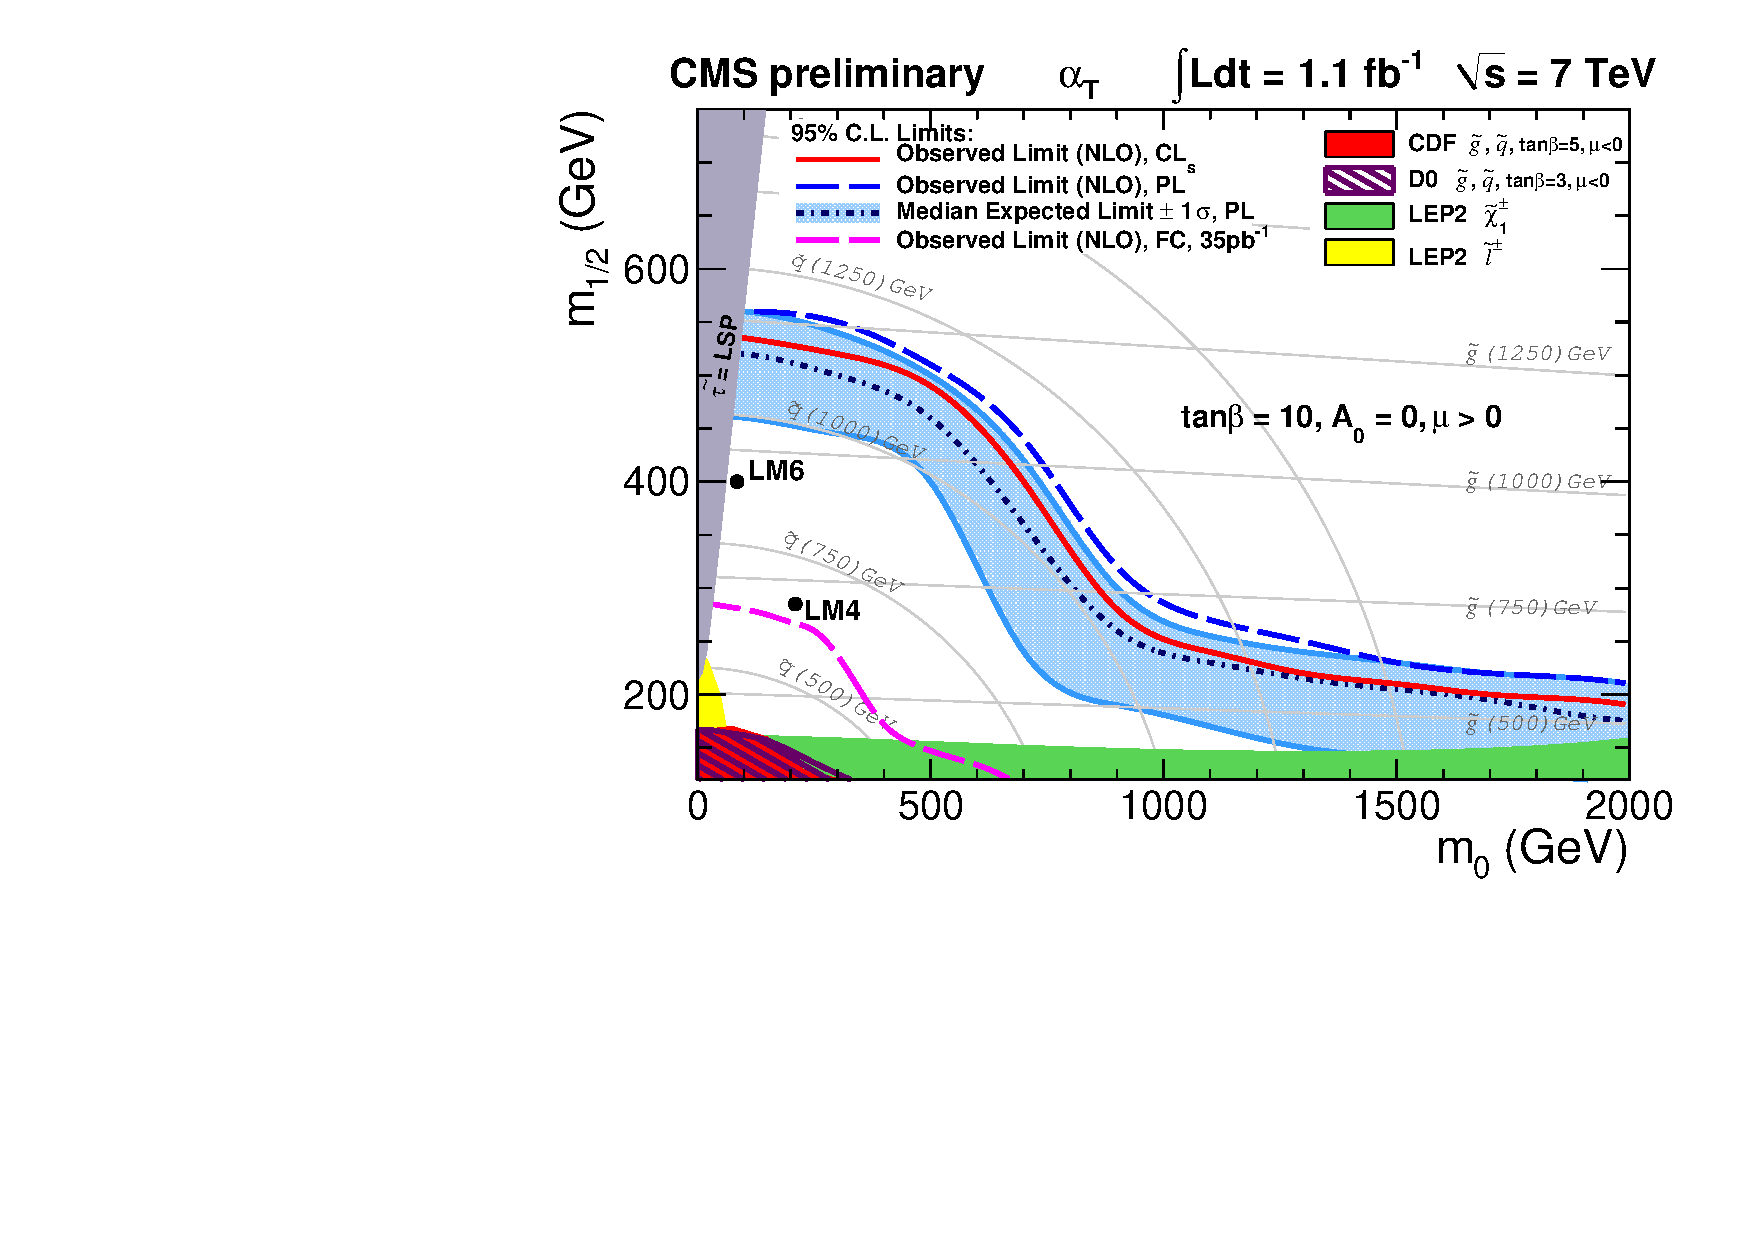
\includegraphics[width = 0.90\textwidth]{Figures/Analysis/PAS/RA1_ExclusionLimit_tanb10_def.pdf}
    \caption{\label{fig:cmssm} Observed and expected 95\% CL exclusion
      contours in the CMSSM ($m_0, m_{1/2}$) plane ($\tan \beta = 10,
      A_0 = 0, \mu > 0$) using NLO signal cross sections using the
      Profile Likelihood (PL) method. The expected limit is shown with
      its 68\% CL range.  The observed limit using the $\cls$ method is
      shown as well.  }
  \end{center}
\end{figure}


\section{Conclusion}

